W~celu określenia czy możliwe jest zbudowanie funkcjonalnej, prywatnej sieci czujnikowej opierając się o~standard LoRa,
przeprowadzony został zestaw badań. Pozwoliły one na dokładniejsze zapoznanie się ze standardem oraz jego możliwościami.
Zbadane zostały elementy podstawowe -- jakość komunikacji pomiędzy modułami, w~celu określenia czy wykorzystanie takiej
sieci nie wiąże się z~większymi problemami niż typowe standardy jak np. ZigBee. Zbadane zostały też parametry sieci
podczas jej pracy -- zasięg komunikacji, zużycie energii. Przeprowadzona została także analiza widmowa, w~celu
zaobserwowania jak wygląda komunikacja w~standardzie LoRa -- celem tego badania była próba zaobserwowania oraz analizy
techniki, jaką standard wykorzystuje do transmisji danych -- tzw. Chirp.

\section{\label{sect:network-comm}Badanie komunikacji w~sieci} Podstawowym badaniem było sprawdzenie poprawności
komunikacji w~dłuższym okresie niż kilka minut. Miało ono na celu określenie czy wybór standardu LoRa jest wyborem
dobrym do prób implementacji sieci czujnikowej. Badanie to było rozszerzeniem testu implementacji, które pozwoliło na
sprawdzenie jakości komunikacji. W~przypadku, gdyby wynik badania pokazał, że sieć ma problemy z~komunikacją, który nie
było widać w~krótkich testach, należałoby przemyśleć czy standard LoRa jest poprawnym wyborem.

Aby otrzymać zestaw danych testowych, moduły pozostały włączone, bez restartowania ich, przez 1~godzinę. Przy ustawieniu
okresu pomiędzy wysyłaniem żądań przez moduł MASTER na 1~minutę dało to 61 pełnych wymian danych w~sieci -- 1~żądanie
przy pierwszym uruchomieniu modułu MASTER oraz 60 podczas pracy modułu na zaimplementowanym zegarze (w sumie 183 żądania
do każdego modułu SLAVE). Średnia odległość pomiędzy modułami podczas badania wynosiła 0.45m (45cm).

\begin{table}[!htbp]
    \centering
    \caption{\label{tab:1h-comm-test}Wyniki przeprowadzonego badania komunikacji w~czasie 1~godziny.}
    \begin{tabular}{@{}lccc@{}}
        \toprule
        Zapytania         & \multicolumn{1}{l}{SLAVE 1} & \multicolumn{1}{l}{SLAVE 2} & \multicolumn{1}{l}{SLAVE 3} \\ \midrule
        W~sumie {[}-{]}   & 183                         & 183                         & 183                         \\
        Nieudane {[}-{]}  & 4                           & 0                           & 1                           \\
        Nieudane {[}\%{]} & 2.19                        & 0                           & 0.55                        \\ \bottomrule
    \end{tabular}
\end{table}

\FloatBarrier
Na podstawie zebranych danych sporządzony został wykres, przedstawiający otrzymane wyniki  -- sumę wysłanych zapytań
oraz ilość, która zakończyła się błędem. Przedstawiony on został na rysunku \ref{img:network-communication-1h}. Kolorem
niebieskim oznaczono sumę wysłanych zapytań, natomiast kolorem pomarańczowym ilość z~brakiem odpowiedzi lub odrzucone
z~powodu błędu. Korzystając z~zebranych danych, możliwe jest zaobserwowanie, że podczas dłuższej komunikacji jedynie
niewielki procent zapytań kończy się błędem, a~wykorzystanie standardu LoRa jest wyborem, pozwalającym na budowanie
sieci czujnikowych.

\begin{figure}[!htbp]
    \centering
    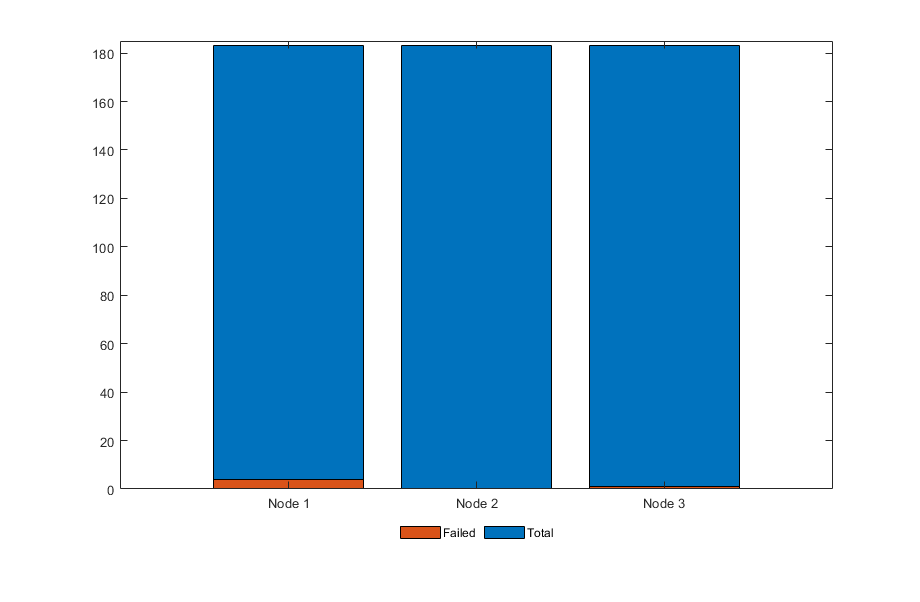
\includegraphics[width=0.8\textwidth]{research/network-communication-1h}
    \caption{\label{img:network-communication-1h}Wykres słupkowy przedstawiający wyniki 1-godzinnego testu komunikacji
        sieci}
\end{figure}

\FloatBarrier
\section{\label{sect:spectral-analisys}Analiza widmowa transmisji w~standardzie LoRa} Aby dokładniej zapoznać się z~tym,
jak działa komunikacja w~standardzie LoRa, wykonana została analiza widmowa transmisji pomiędzy modułami sieci.
Wykorzystane tutaj zostało narzędzie pozwalające na badanie fal radiowych bazujące na SDR (ang. \textsl{Software Defined
    Radio}) -- Hack RF One oraz darmowe, udostępnione w~charterze open source, oprogramowanie \textsl{gqrx} na platformę
Linux. Celem tego badania była obserwacja spektrum sygnałów radiowych w~okolicach częstotliwości, na jakich operuje
LoRa, oraz próba zaobserwowania czy możliwe jest metodą tą zobaczenie pojedynczych chirpów podczas transmisji.
Stanowisko testowe zostało wykorzystane także do zebrania zestawu próbek I/Q, które, w~późniejszym czasie, zostały
poddane analizie wykorzystując do tego środowisko MATLAB.

\subsection{\label{sect:spectral-in-gqrx}Obserwacje transmisji w~oprogramowaniu \textsl{gqrx}} Moduły zostały ustawione
na stanowisku testowym, odległość pomiędzy nimi podczas badania wynosiła, podobnie jak w~przypadku badania komunikacji,
około 0.45m. W~odległości około 1m od ustawionej sieci znajdowała się antena podłączona do Hack RF One. Oprogramowanie
\textsl{gqrx} ustawione zostało w~taki sposób, aby móc odczytywać w~nim dane zbierane przez urządzenie -- rozmiar okna
FFT na 1048576 próbek (maksymalna wartość dostępna w~programie), co dawało rozdzielczość pasma przenoszenia 1Hz oraz
częstotliwość odświeżania na 60fps (ang. \textsl{frames per second} -- klatek na sekundę, maksymalna dostępna). Na tak
przygotowanym stanowisku testowym uruchomione zostały moduły. Aby uzyskać lepszą dokładność obserwacji, na modułach
wyłączona została funkcjonalność pracy na zegarze, a~transmisja uruchamiana była każdorazowo ręcznie (wykorzystując
przycisk na module MASTER).

Pierwsze próby obserwacji komunikacji przeprowadzone zostały na podstawowych ustawieniach modułów -- najniższa wartość
Spreading Factor, SF7 (7 bitów na symbol), pasmo 125kHz, radio coding rate, CR, 4/5. Takie parametry pozwalają sieci na
szybką komunikację, jednakże w~przypadku analizy widmowej nie pozwoliły one na dobrą obserwację transmisji. W~tym celu
parametr Spreading Factor przestawiony został na wartość maksymalną, SF12 (12 bitów na symbol). Spowodowało to
wydłużenie czasu każdej transmisji i~jednocześnie pozwoliło na lepszą obserwację. Korzystając ze zmodyfikowanych
parametrów, wykonane zostało kilkanaście transmisji i~w tym czasie obserwowane było, jak wygląda ich widmo. Rys.
\ref{img:waterfall-full-mid-transmission} przedstawione zostało, jak wyglądała obserwowana transmisja (tutaj: pełna sieć,
w~trakcie transmisji przez jeden z~modułów).

\begin{figure}[!htbp]
    \centering
    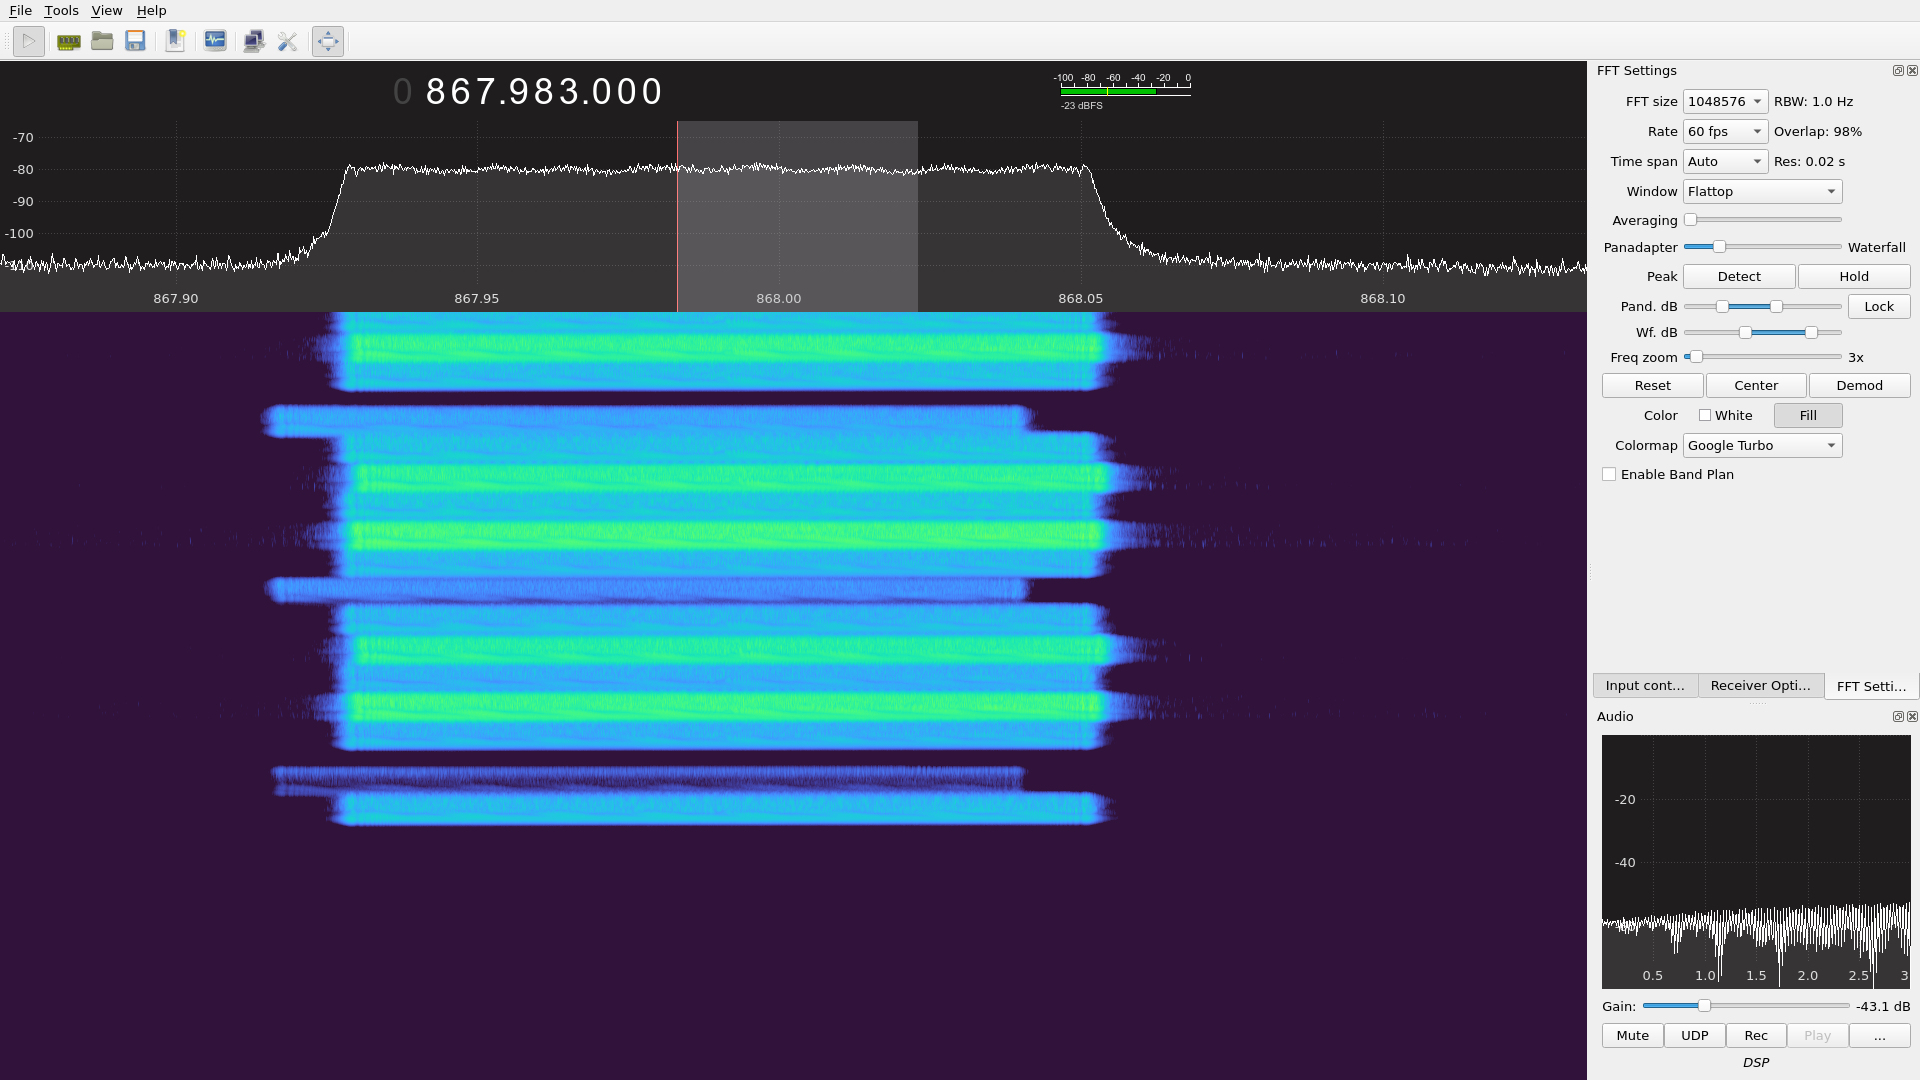
\includegraphics[width=0.9\textwidth]{research/waterfall-full-mid-transmission}
    \caption{\label{img:waterfall-full-mid-transmission}Zrzut ekranu z~programu pokazujący obserwowane transmisje}
\end{figure}

\FloatBarrier
Podczas badania wykonane zostały transmisje w~kilku konfiguracjach -- pełna sieć, 2~moduły SLAVE oraz 1~moduł SLAVE.
W~tym czasie wykonywane zostały zrzuty ekranów widoku z~programu \textsl{gqrx}. Na rys.
\ref{img:waterfall-full-no-timeouts}, \ref{img:waterfall-full-with-timeouts}, \ref{img:waterfall-one-slave} oraz
\ref{img:waterfall-two-slave} przestawione zostały wyniki obserwacji.

\begin{figure}[!htbp]
    \centering
    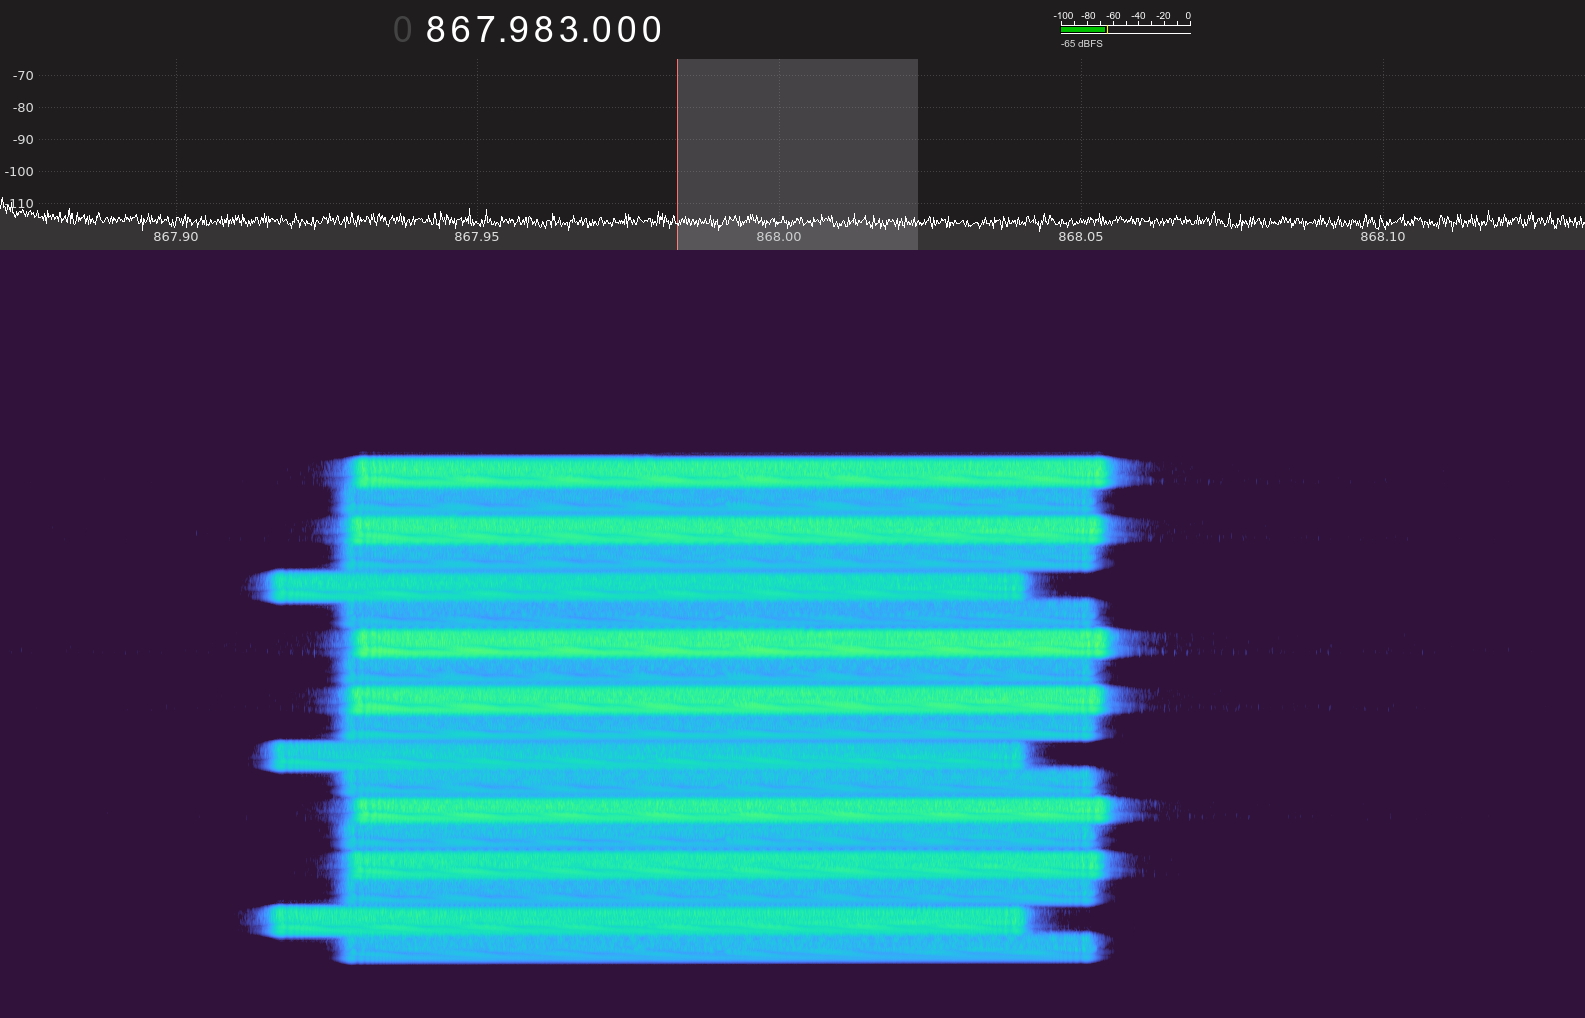
\includegraphics[width=0.9\textwidth]{research/waterfall-full-network-no-timeouts}
    \caption{\label{img:waterfall-full-no-timeouts}Widok na komunikację pełnej sieci, bez wystąpienia problemów
        z~komunikacją}
\end{figure}

\begin{figure}[!htbp]
    \centering
    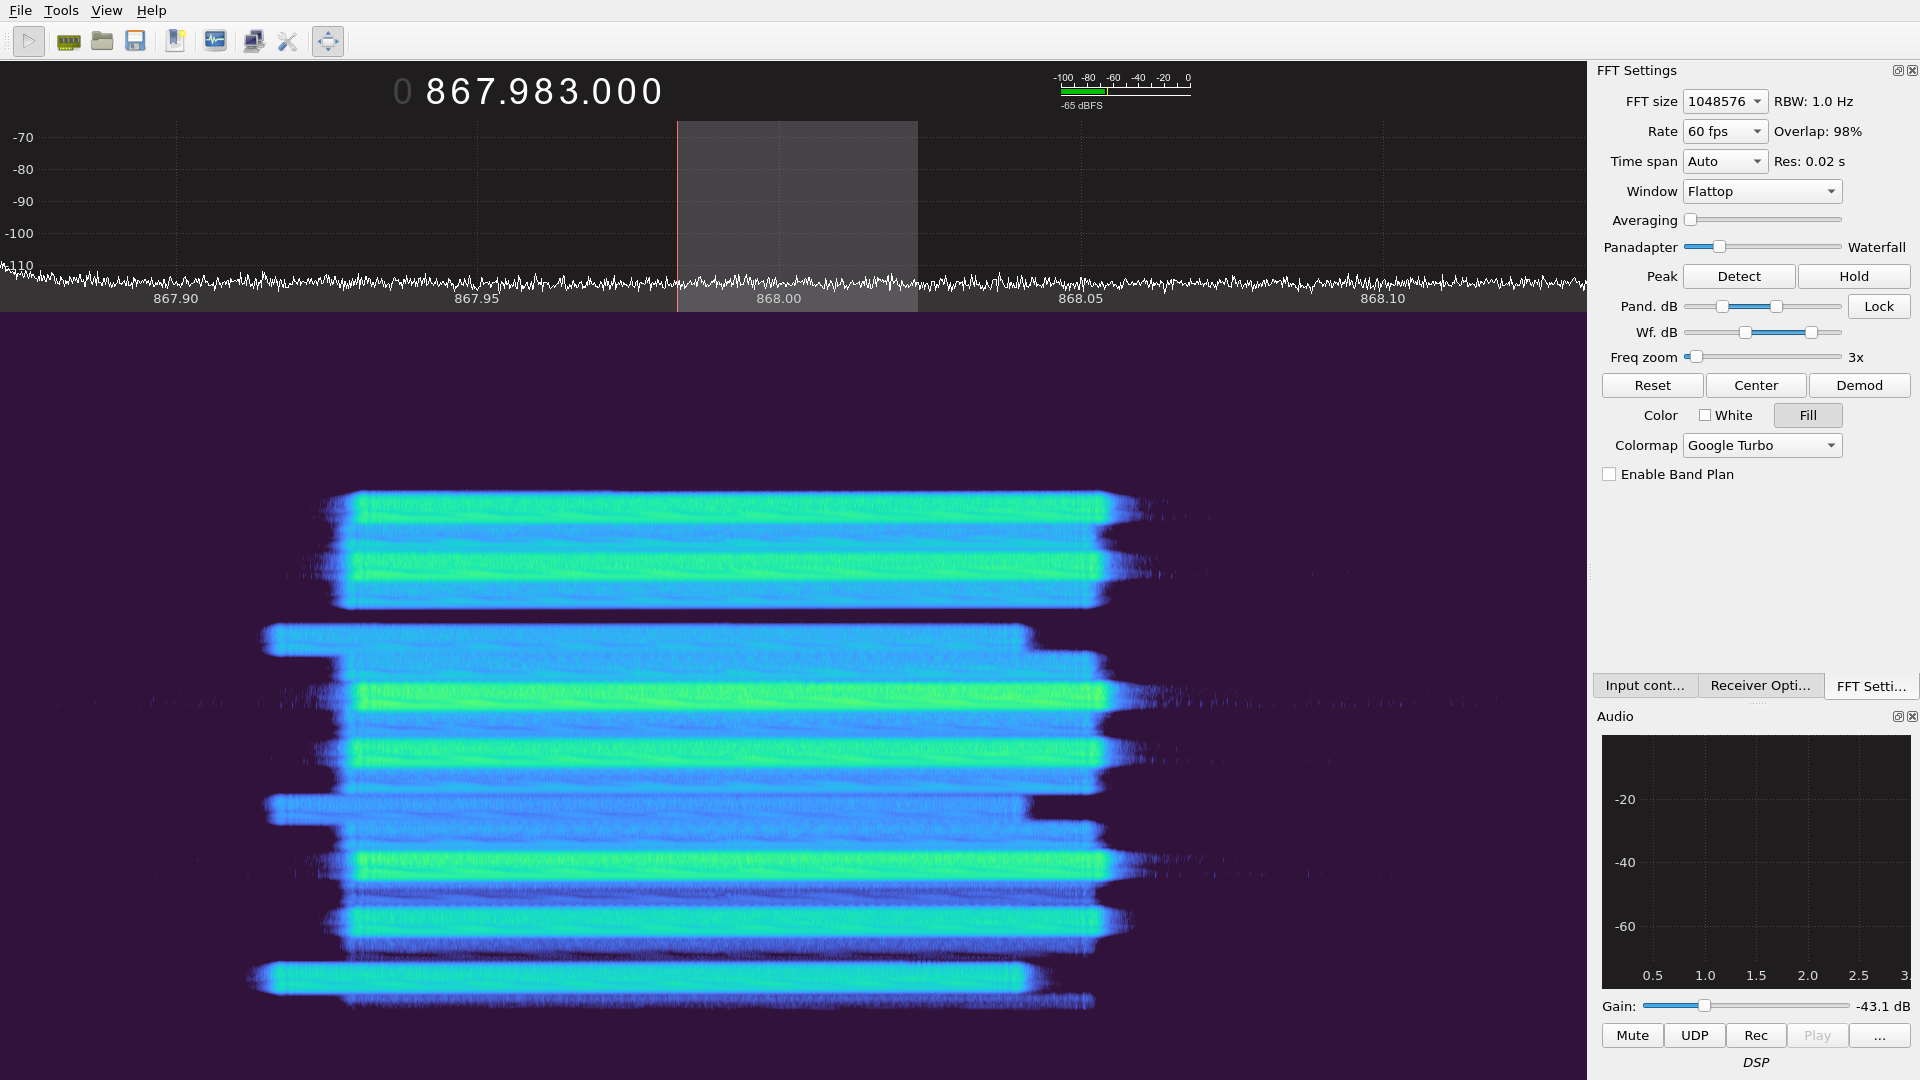
\includegraphics[width=0.9\textwidth]{research/waterfall-full-network-with-timeouts}
    \caption{\label{img:waterfall-full-with-timeouts}Widok na komunikację pełnej sieci, z~widocznymi przerwami, gdy
        jeden z~modułów nie odpowiedział na zapytanie}
\end{figure}

\begin{figure}[!htbp]
    \centering
    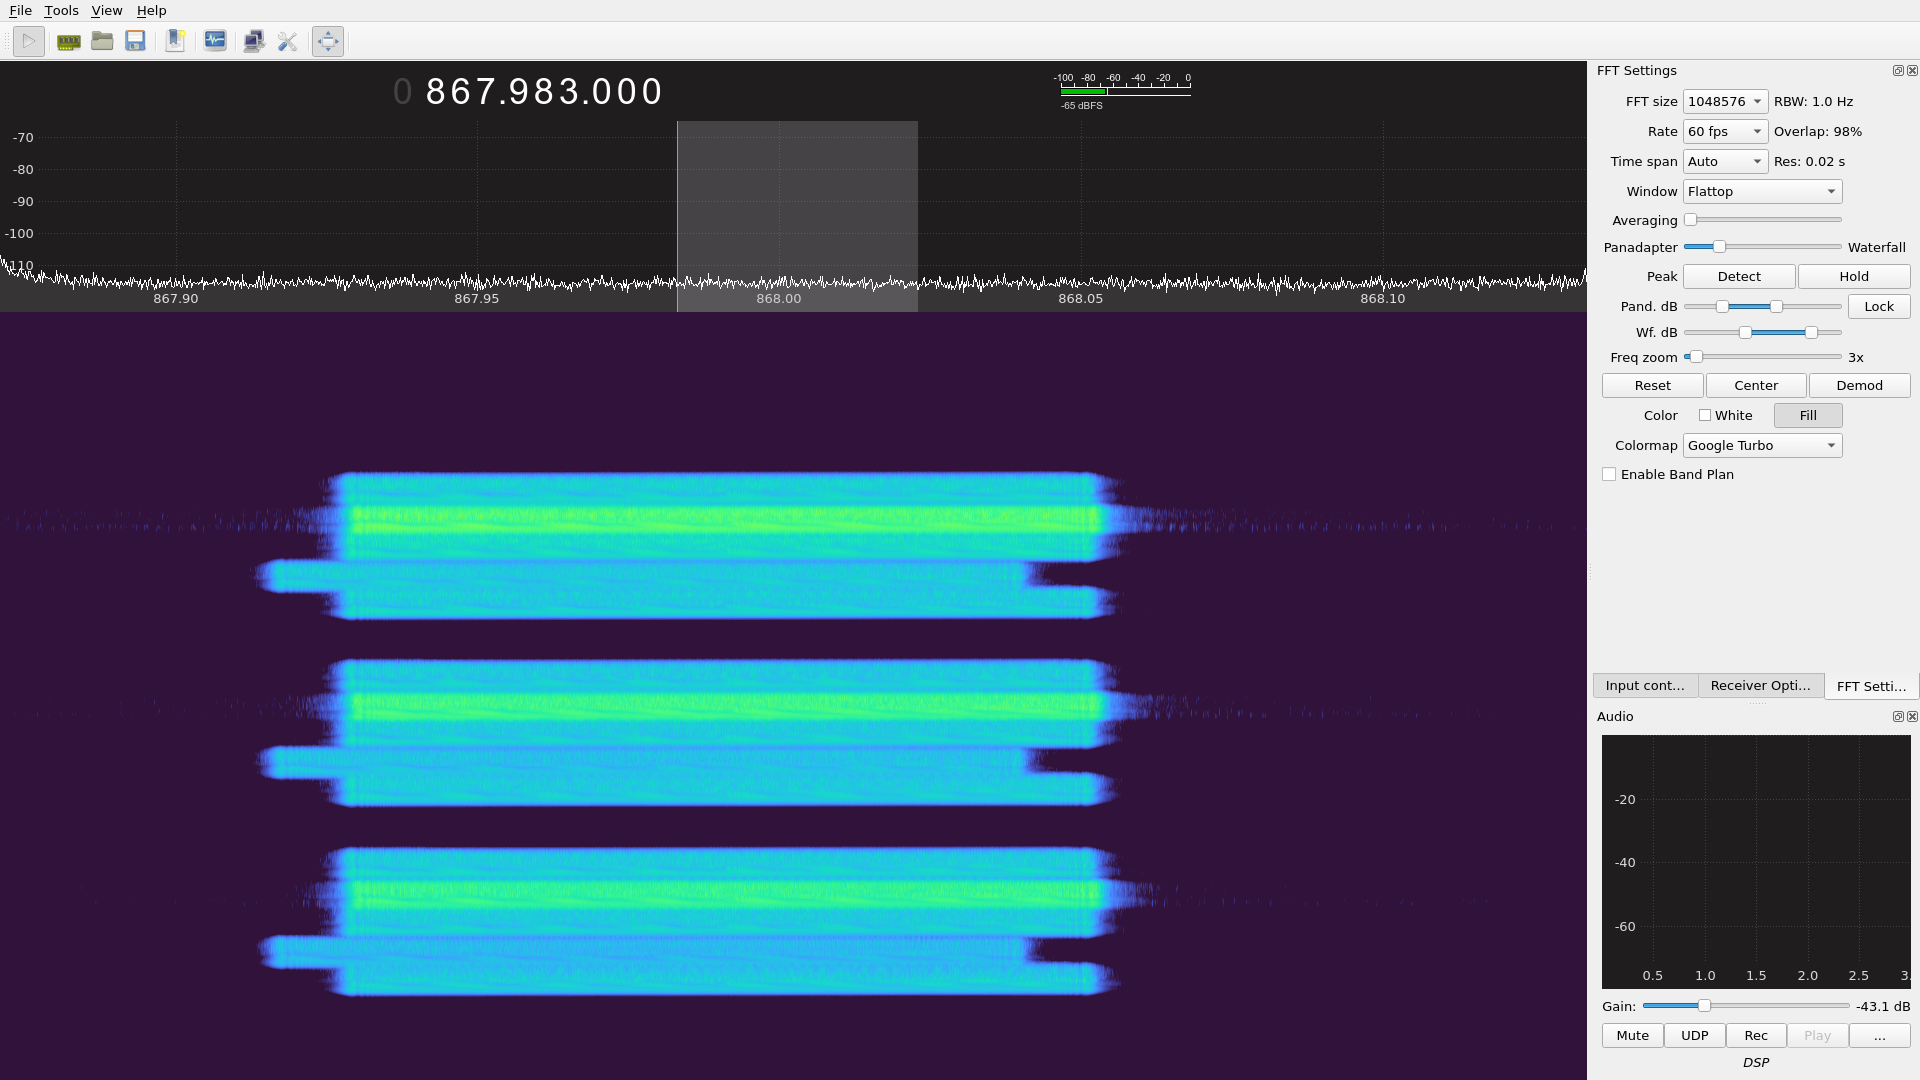
\includegraphics[width=0.9\textwidth]{research/waterfall-two-slave-network}
    \caption{\label{img:waterfall-one-slave}Widok na komunikację w~sieci dwoma modułami SLAVE włączonymi, a~jednym
        wyłączonym}
\end{figure}

\begin{figure}[!htbp]
    \centering
    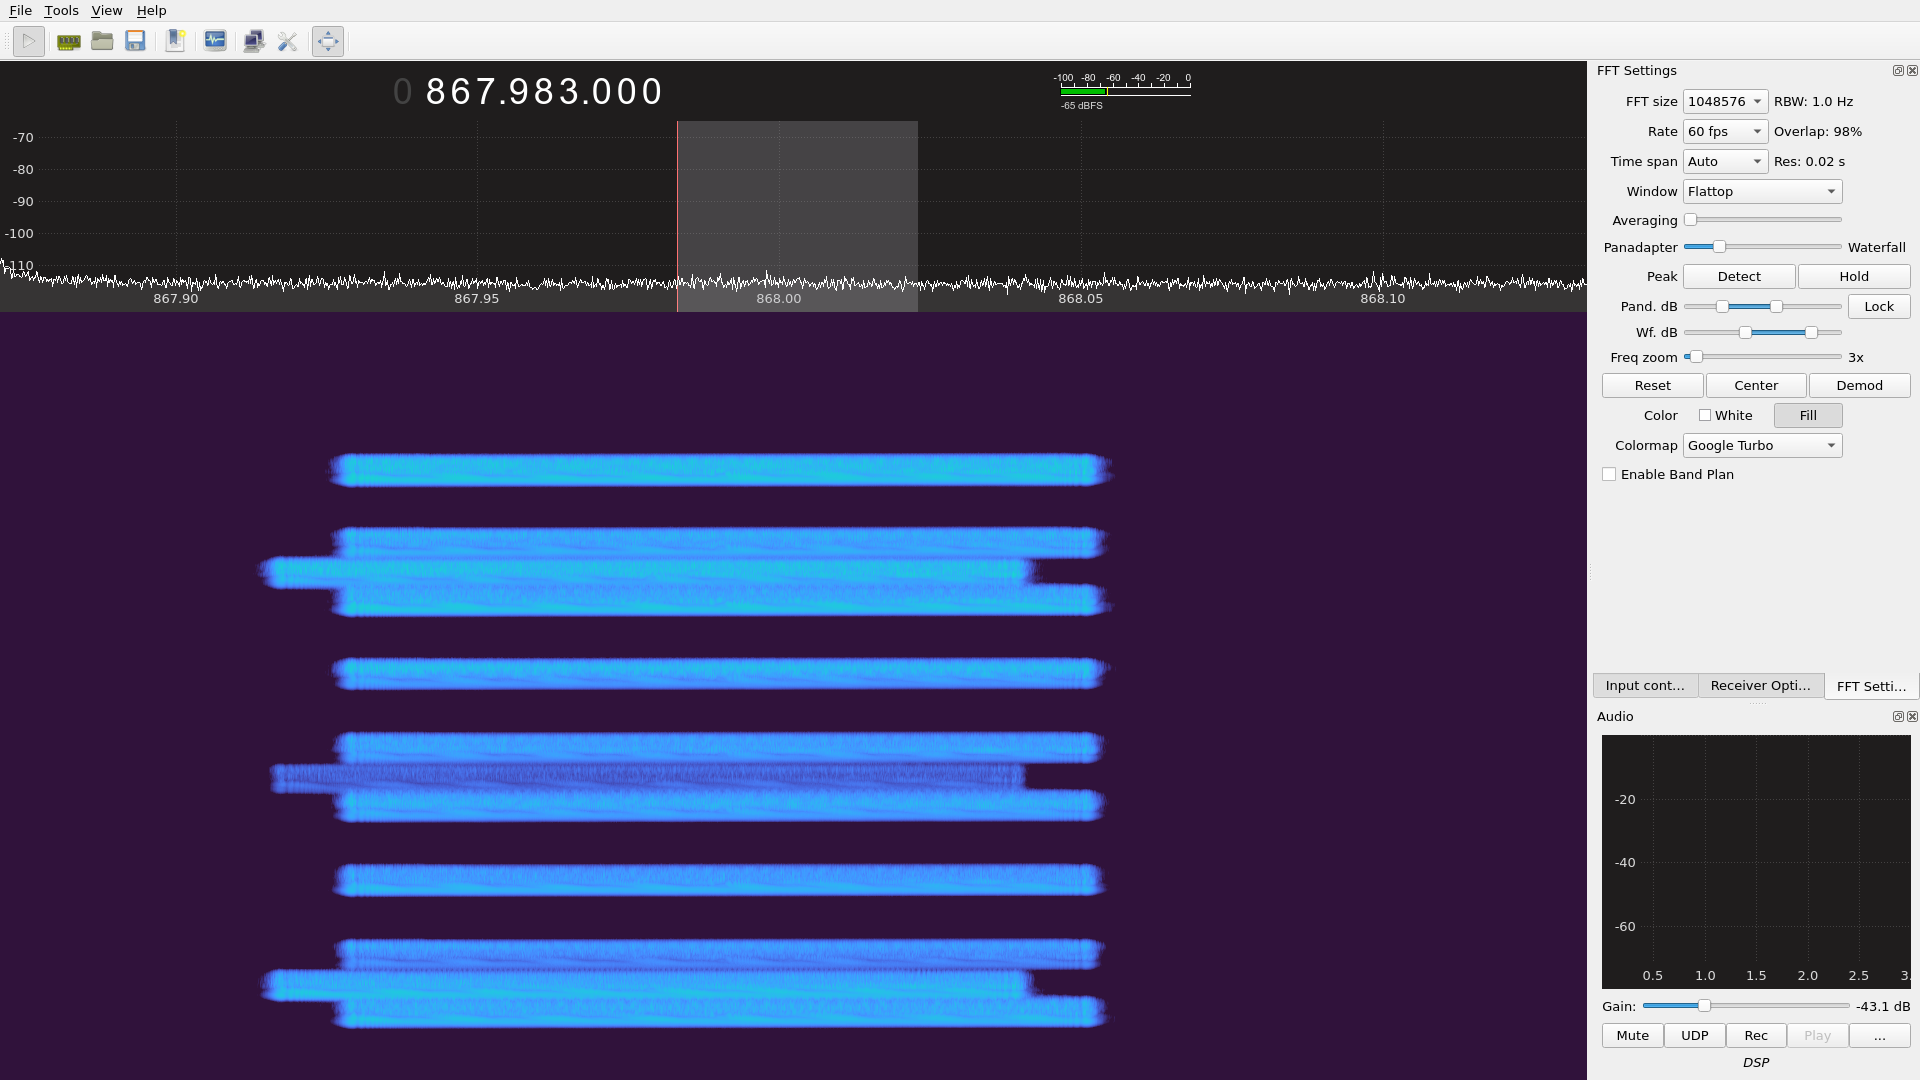
\includegraphics[width=0.9\textwidth]{research/waterfall-one-slave-network}
    \caption{\label{img:waterfall-two-slave}Widok na komunikację w~sieci z~tylko jednym modułem SLAVE włączonymi}
\end{figure}

\FloatBarrier
W~przypadku, gdzie udało się zaobserwować pełną komunikację, gdzie nie wystąpiły żadne problemy, wyraźnie widać 9~wymian
pomiędzy modułami (18 transmisji). Natomiast w~przypadkach, gdy pojawił się błąd, bądź dany moduł był wyłączony wyraźnie
widać to w~zaobserwowanym zapisie. Niestety w~przypadku obserwacji wykorzystując do tego program \textsl{gqrx} nie udało
zaobserwować się pojedynczych elementów każdej transmisji (pojedynczych chirpów, preambuły czy wysyłanych symboli). Jest
to związane z~ograniczeniami oprogramowania co do maksymalnej szybkości odświeżania widoku na ekranie.

Poza obserwacją tzw. wykresów wodospadowych (pokazujących zmiany w~widmie w~czasie) udało się także zebrać zapisy
rozkładu częstotliwości sygnałów podczas transmisji wykonywanych przez moduły. Przedstawione zostało to na rys.
\ref{img:frequency-graph-no-transmission}, \ref{img:frequency-graph-master-request} oraz
\ref{img:frequency-graph-slave-response}. Ciekawym faktem jest tutaj widoczna w~przypadku transmisji z~modułów SLAVE
wyższa moc sygnałów. Spowodowane to było najprawdopodobniej faktem, że były umieszczone bliżej anteny podłączonej do
urządzenia zbierającego dane.

\begin{figure}[!htbp]
    \centering
    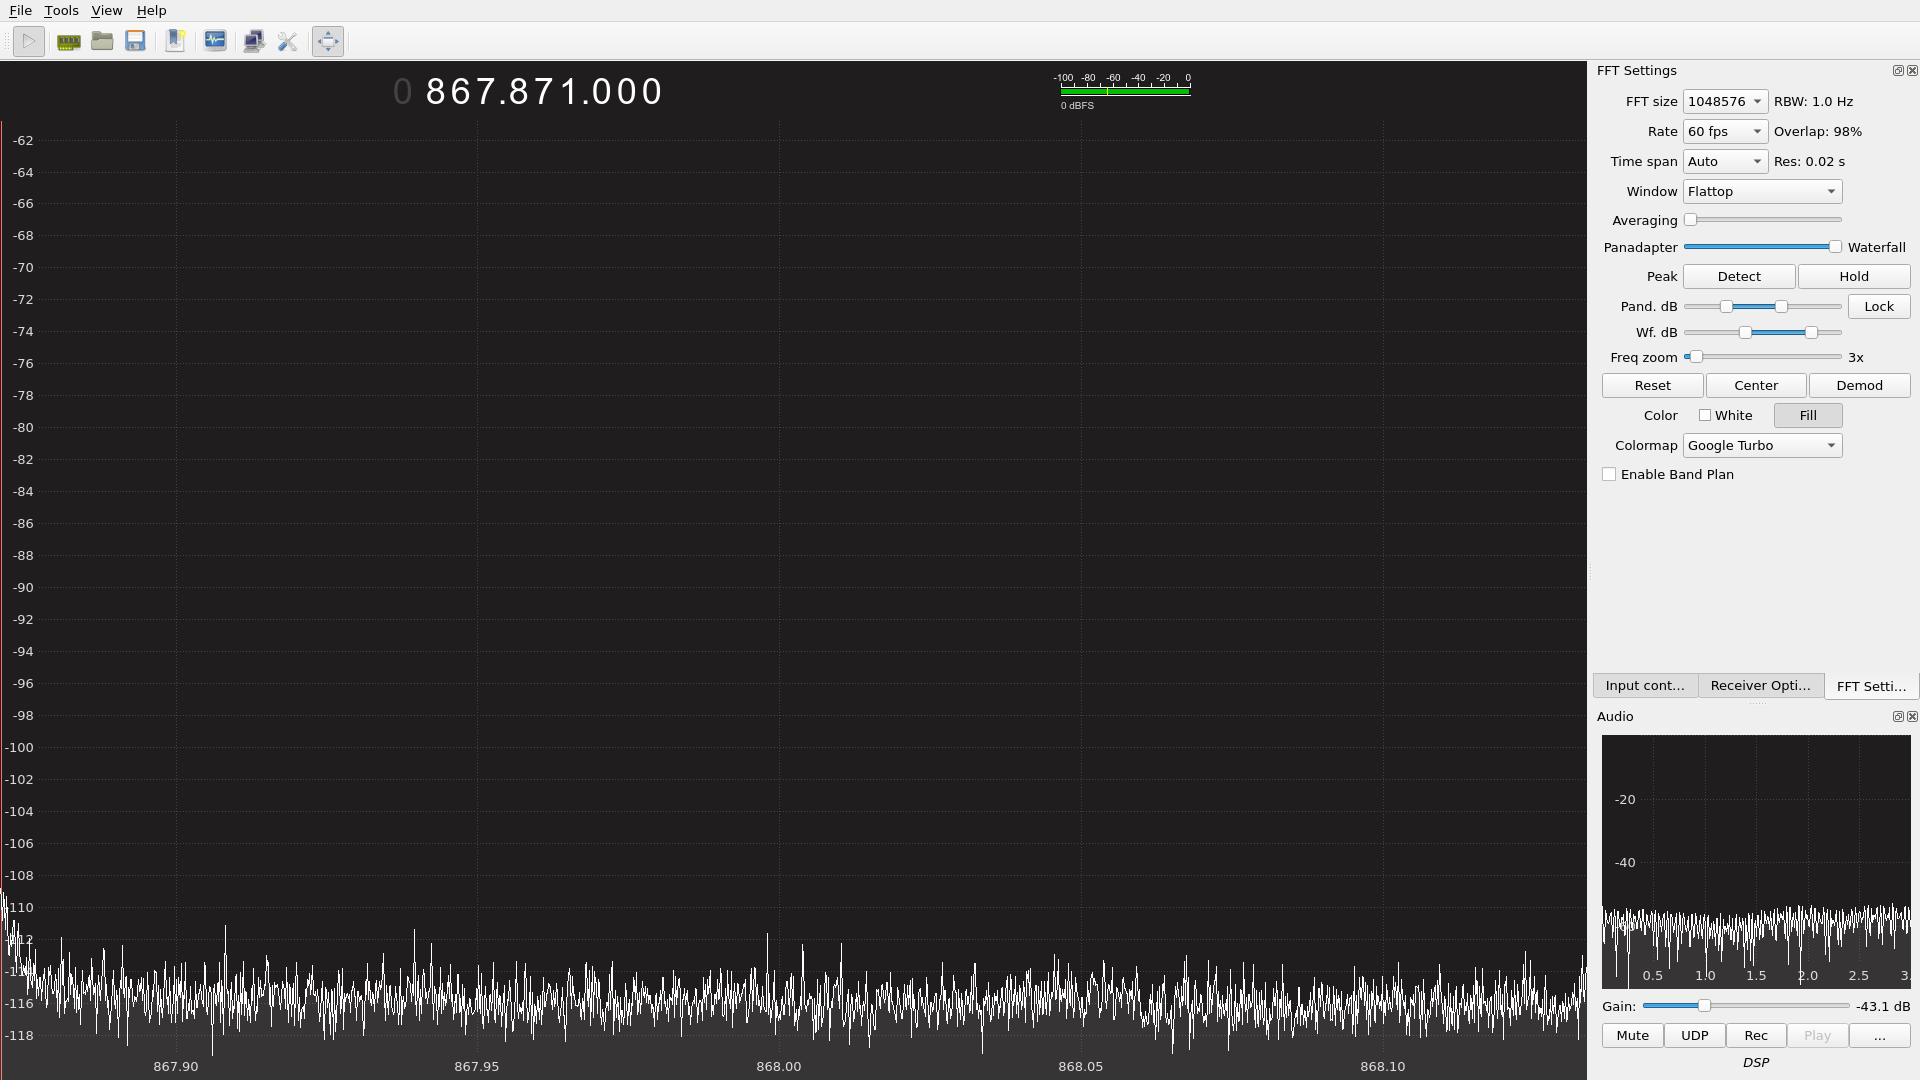
\includegraphics[width=0.9\textwidth]{research/frequency-graph-no-transmission}
    \caption{\label{img:frequency-graph-no-transmission}Widok spektrum częstotliwości, gdy żaden z~modułów nie transmituje}
\end{figure}

\begin{figure}[!htbp]
    \centering
    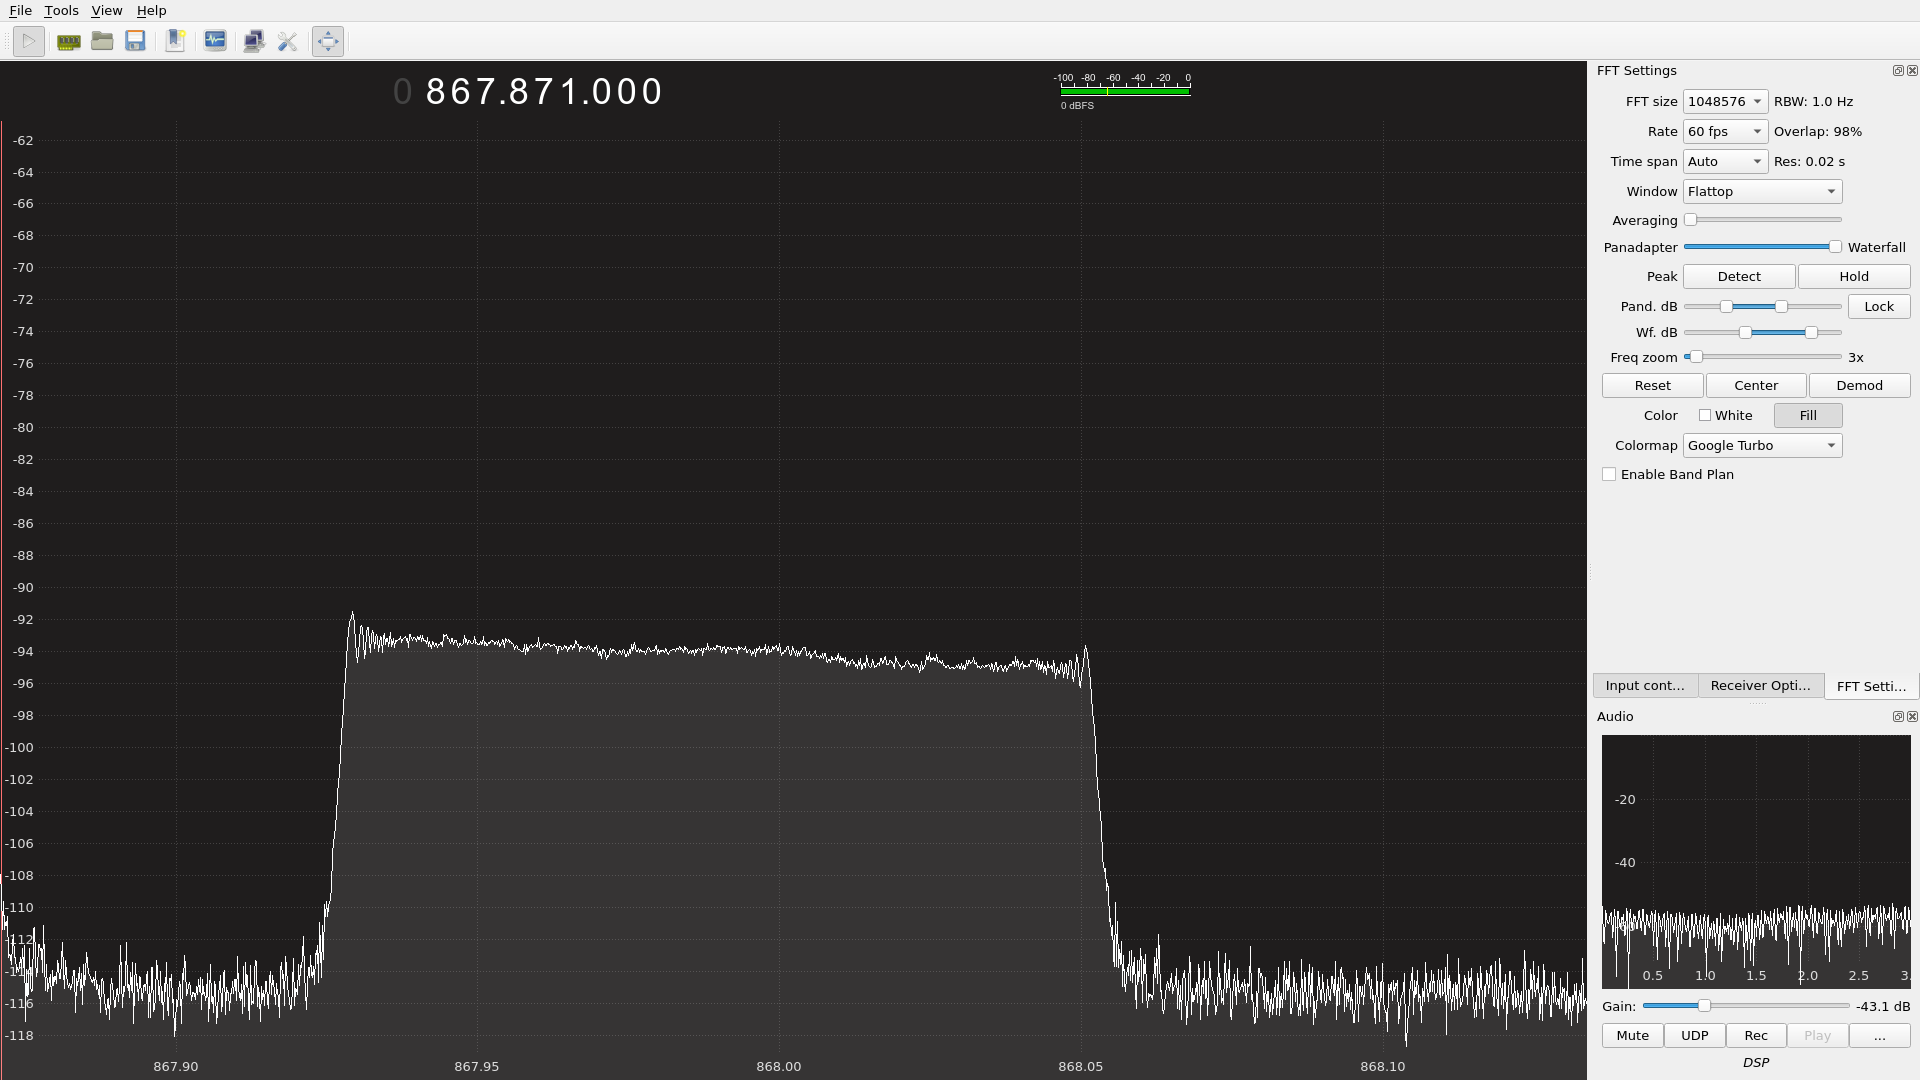
\includegraphics[width=0.9\textwidth]{research/frequency-graph-master-request}
    \caption{\label{img:frequency-graph-master-request}Widok spektrum częstotliwości podczas transmisji modułu MASTER}
\end{figure}

\begin{figure}[!htbp]
    \centering
    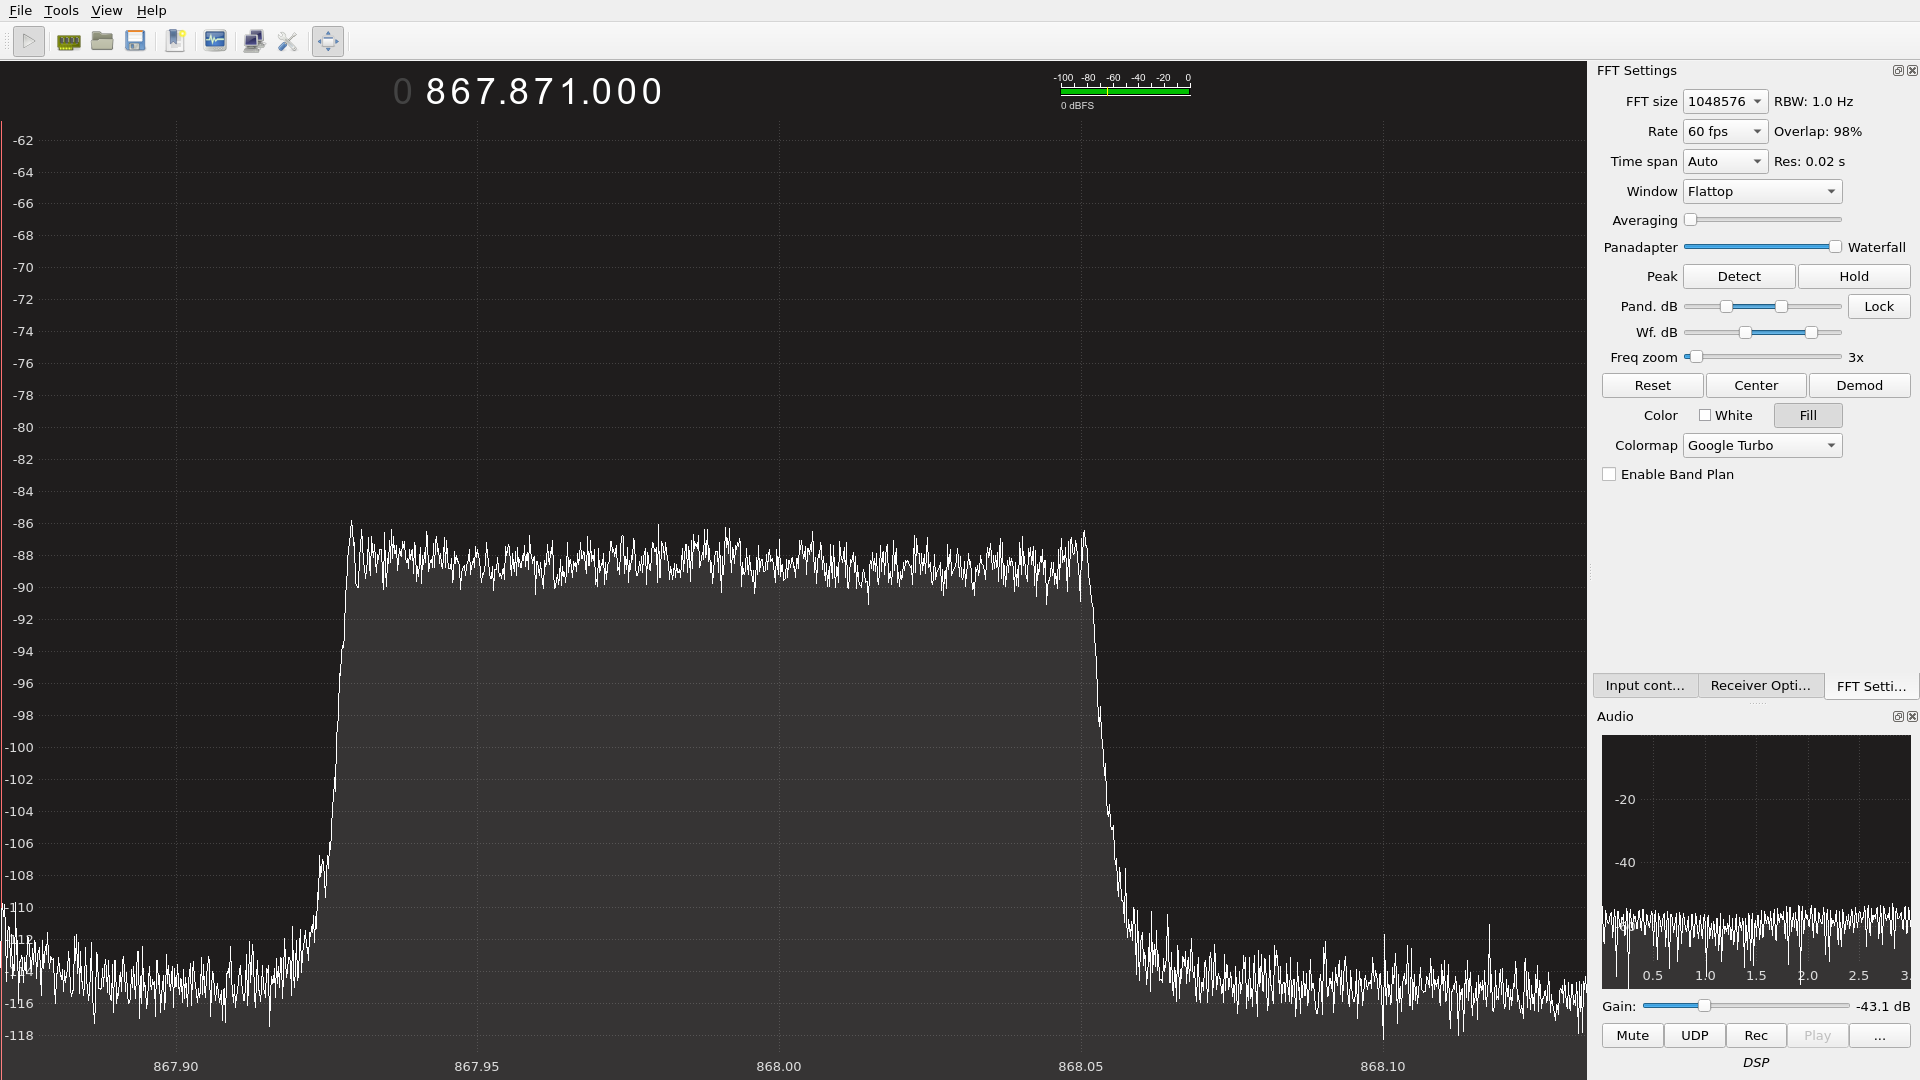
\includegraphics[width=0.9\textwidth]{research/frequency-graph-slave-response}
    \caption{\label{img:frequency-graph-slave-response}Widok spektrum częstotliwości podczas transmisji modułów SLAVE}
\end{figure}

\FloatBarrier
\subsection{\label{sect:iq-data-gqrx}Analiza zapisów danych I/Q zebranych \textsl{gqrx}} Ponieważ wykresy obserwowane
bezpośrednio w~oprogramowaniu \textsl{gqrx} nie pozwalały na analizę przesyłanych transmisji z~modułów, wykorzystana
została funkcja zapisu rejestrowanych danych do postaci I/Q (ang. \textsl{In-phase and quadrature components}) do plików
RAW. W~celu późniejszej analizy danych wykonane zostały 3~zapisy pełnych wymian danych w~sieci w~różnych konfiguracjach,
z~parametrami modułów ustawionych na podstawowych wartościach z~wyjątkiem Spreading Factor. Parametr ten ustawiony
został na wartość maksymalną (SF12, 12 bitów na symbol), tak aby uzyskać najlepsze szanse na analizę transmisji.

Dane I/Q to metoda opisu wielkości i~danych fazowych rejestrowanego sygnału, gdzie falę sinusoidalną można przedstawić
w~formie współrzędnych biegunowych \cite{ni-iq-data} korzystając z~równania:
\begin{equation}
    f(t) = A\cos{2\pi{ft}+\varphi}
\end{equation}
Zarejestrowane w~ten sposób dane (sinusoidę z~modulacją) można rozłożyć na dwie sinusoidy z~modulacją amplitudy, które
przesunięte są względem siebie w~fazie o ${\pi}/2$ radianów (90 stopni). Zarejestrowaną falę można wówczas przedstawić
w~złożonym układzie współrzędnych kartezjańskich, w~postaci składowych rzeczywistej i~urojonej, korzystając z~równań:
\begin{equation}
    I(t) = A\cos{\varphi}\cos{2\pi{ft}} \quad\text{(Składowa rzeczywista)}
\end{equation}
\begin{equation}
    Q(t) = A\sin{\varphi}\sin{2\pi{ft}} \quad\text{(Składowa urojona)}
\end{equation}

Korzystając z~zarejestrowanych zapisów, gdzie każdy miał długość około 25 sekund i~składał się z~około 25 milionów
próbek (związane z~ustawionym oknem FFT, milion próbek na sekundę) wykonana została ich analiza w~środowisku MATLAB.
Napisana została funkcja pozwalająca na generowanie spektrogramów pełnego zarejestrowanego sygnału oraz spektrogramów
zbliżenia na konkretne, wyznaczone, elementy. Kod źródłowy przedstawiony został na listingach
\ref{lst:matlab-spectrogram-zoom-1}, \ref{lst:matlab-spectrogram-zoom-2} oraz \ref{lst:matlab-spectrogram-zoom-3}
(przedstawiają kolejno: argumenty wejściowe funkcji, właściwe generowanie spektrogramów oraz funkcje pomocnicze do
ładowania danych z~plików RAW i~eksportu wygenerowanych wykresów).

\lstinputlisting[
    language=matlab,
    linerange={3-12},
    caption={Funkcja do analizy danych I/Q w~MATLAB -- argumenty wejściowe},
    label={lst:matlab-spectrogram-zoom-1},
    float=htbp
]{gqrx-spectrograms/spectrogramzoom.m}

\lstinputlisting[
    language=matlab,
    linerange={14-40},
    caption={Funkcja do analizy danych I/Q w~MATLAB -- generowanie pełnego spektrogramu oraz zbliżenia na wycinek},
    label={lst:matlab-spectrogram-zoom-2},
    float=htbp
]{gqrx-spectrograms/spectrogramzoom.m}

\lstinputlisting[
    language=matlab,
    linerange={43-57},
    caption={Funkcja do analizy danych I/Q w~MATLAB -- funkcje pomocnicze},
    label={lst:matlab-spectrogram-zoom-3},
    float=htbp
]{gqrx-spectrograms/spectrogramzoom.m}

Argumentami wejściowymi funkcji są: plik wejściowy (zawierający dane I/Q), ścieżka oraz nazwa pliku, gdzie wygenerowany
wykres ma zostać zapisany, zasięg próbek, na jakim ma zostać wykonane zbliżenie oraz dodatkowe parametry do funkcji
\texttt{spectrogram} -- wielkość okna, częstotliwość próbkowania, liczba nakładających się próbek, liczba punktów do
dyskretnej transformaty Fouriera.

\FloatBarrier
Funkcja pomocnicza, wykorzystywana do ładowania plików RAW, bazuje na równianach opisujących składowe rzeczywistą
i~urojoną. Plik zostaje otwarty w~momencie wywołania funkcji, a~jego zawartość odczytana w~postaci 32-bitowych wartości
zmiennoprzecinkowych (float32) z~najbardziej znaczącym bajtem jako pierwszym (ang. \textsl{Big endian}). Następnie
zawartość pliku ładowana jest do pamięci programu, modyfikując je do postaci złożonej (ang. \textsl{Complex}).

Generowanie spektrogramów wykorzystuje wbudowaną funkcję \texttt{spectrogram}. W~przypadku generowania wykresu dla
całego sygnału wykorzystywane są tylko argumenty wejściowe. Dodatkowo na podstawie wprowadzonych wartości, gdzie ma
zostać wykonane zbliżenie, na wykresie rysowane są linie pionowe na osi X. Korzystając z~długości (wielkości) tablicy
danych wejściowych, ustalane są ilość oraz rozstawienie podziałki. Natomiast w~przypadku wykresu zbliżenia, pierwszym
elementem jest wyznaczenie zakresu próbek, na podstawie których wygenerowany ma zostać spektrogram. Korzystając z~tych
dodatkowych zmiennych oraz pozostałych argumentów wejściowych generowany jest spektrogram zbliżenia. Ostatnim krokiem
w~funkcji jest eksport wykresu do pliku. Wykorzystywana jest do tego zaimplementowana funkcja pomocnicza
\texttt{exportfigure}. Zdefiniowane w~niej zmienne wykorzystywane są do zachowania poprawnych proporcji, tak aby wykres
miał największą możliwą czytelność.

\FloatBarrier
Korzystając z~zaimplementowanej funkcji, wygenerowane zostały spektrogramy jednego z~zarejestrowanych sygnałów, stosując
zwiększające przybliżenie, w~celu uzyskania jak najlepszego widoku na pojedynczą transmisję. Wygenerowane wykresy
przedstawione zostały przedstawione na rys. \ref{img:signal1-level1}, \ref{img:signal1-level2}, \ref{img:signal1-level3}
oraz \ref{img:signal1-level4} (zbliżenia w~czasie 2.5s a 6s, pokazujące 3~transmisje, do 3.6s a 4.6s, pokazując
dokładniej 1~transmisję).

\begin{figure}[!htbp]
    \centering
    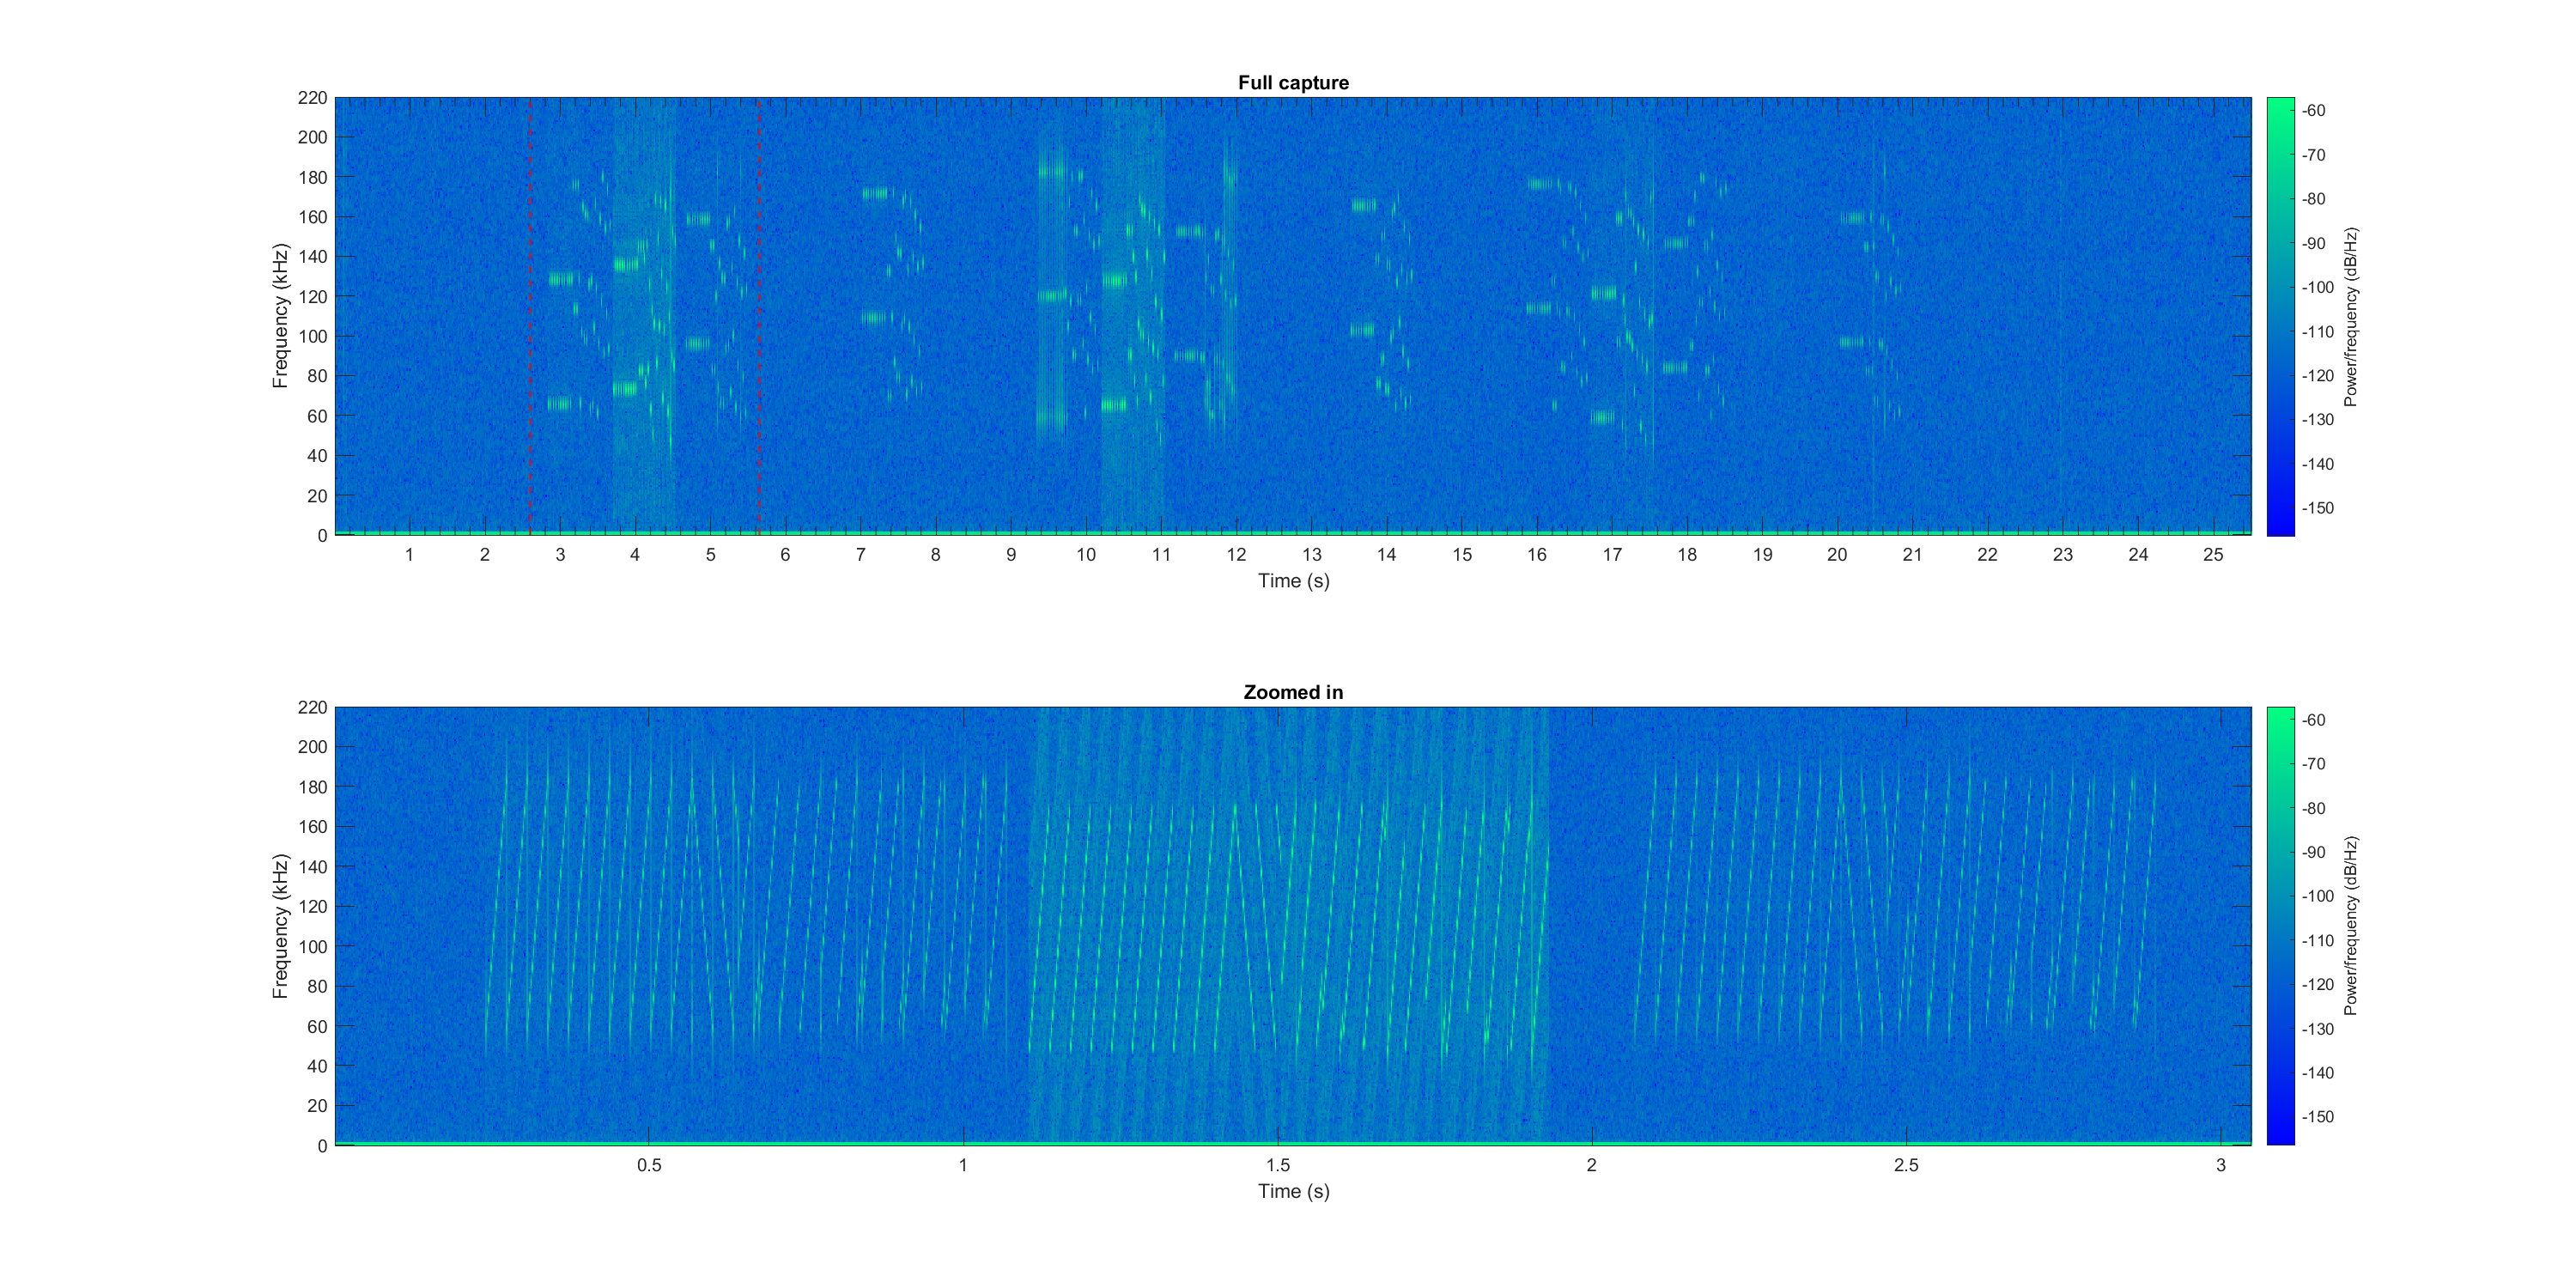
\includegraphics[width=\textwidth]{research/gqrx/zoom-win1024-sig1-lvl1}
    \caption{\label{img:signal1-level1}Spektrogram sygnałów z~pierwszej próbki wraz ze zbliżeniem między 2.5s a 5.5s}
\end{figure}

\begin{figure}[!htbp]
    \centering
    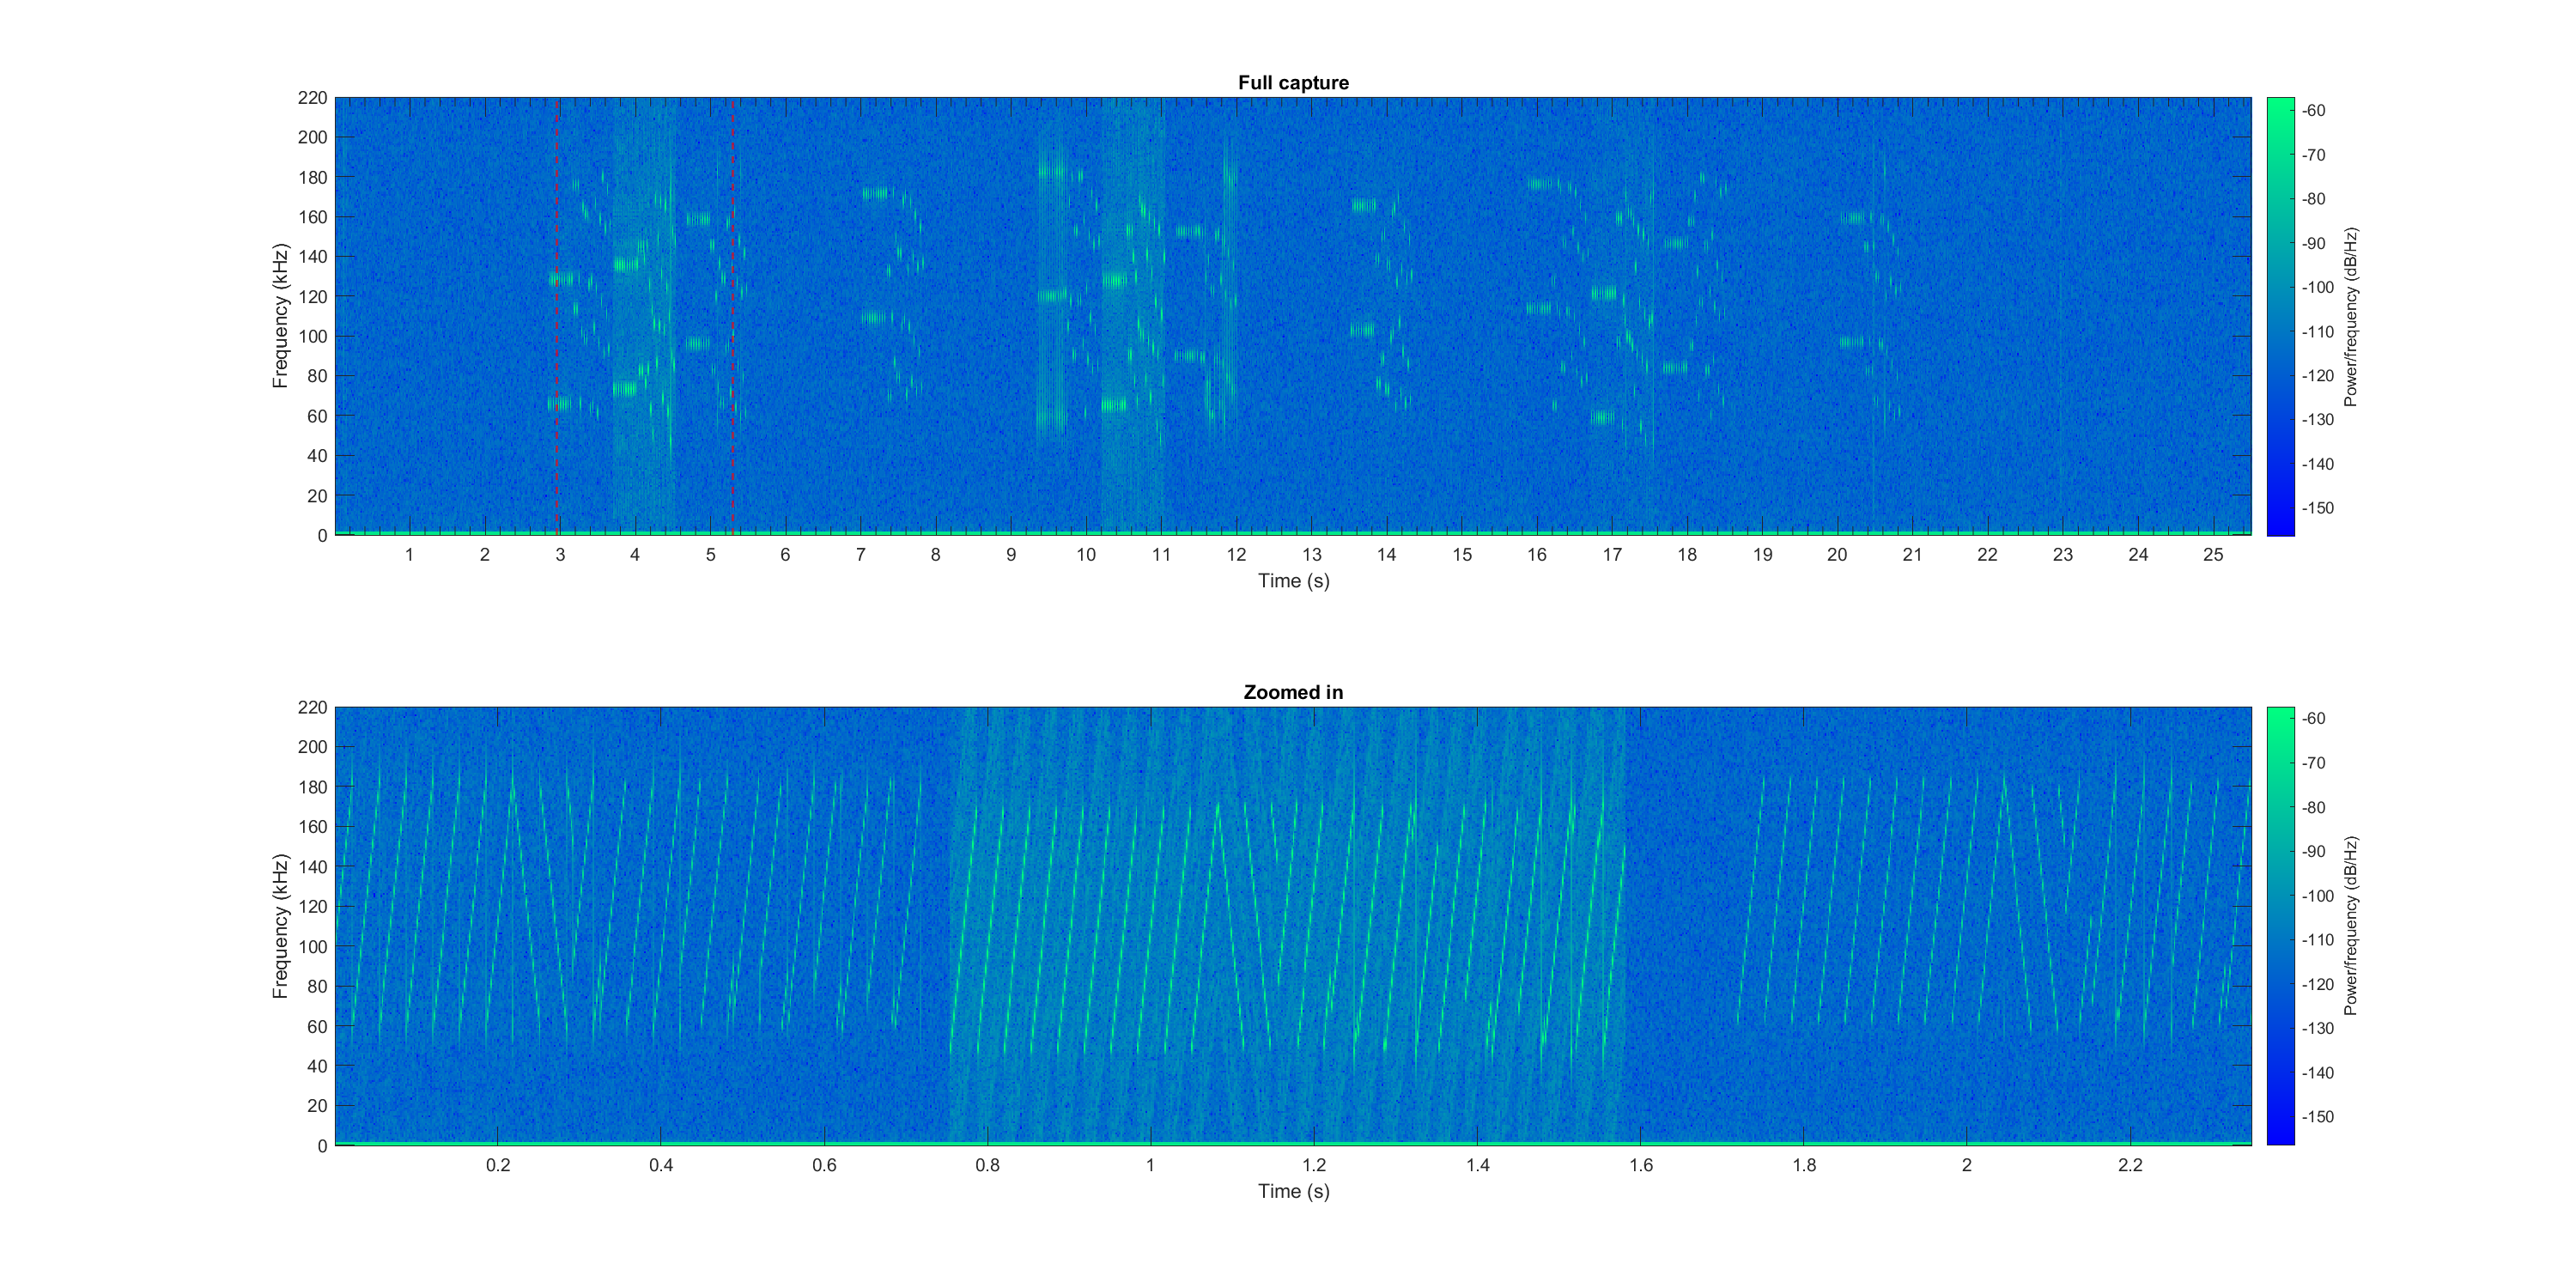
\includegraphics[width=\textwidth]{research/gqrx/zoom-win1024-sig1-lvl2}
    \caption{\label{img:signal1-level2}Spektrogram sygnałów z~pierwszej próbki wraz ze zbliżeniem między 3s a 5.1s}
\end{figure}

\begin{figure}[!htbp]
    \centering
    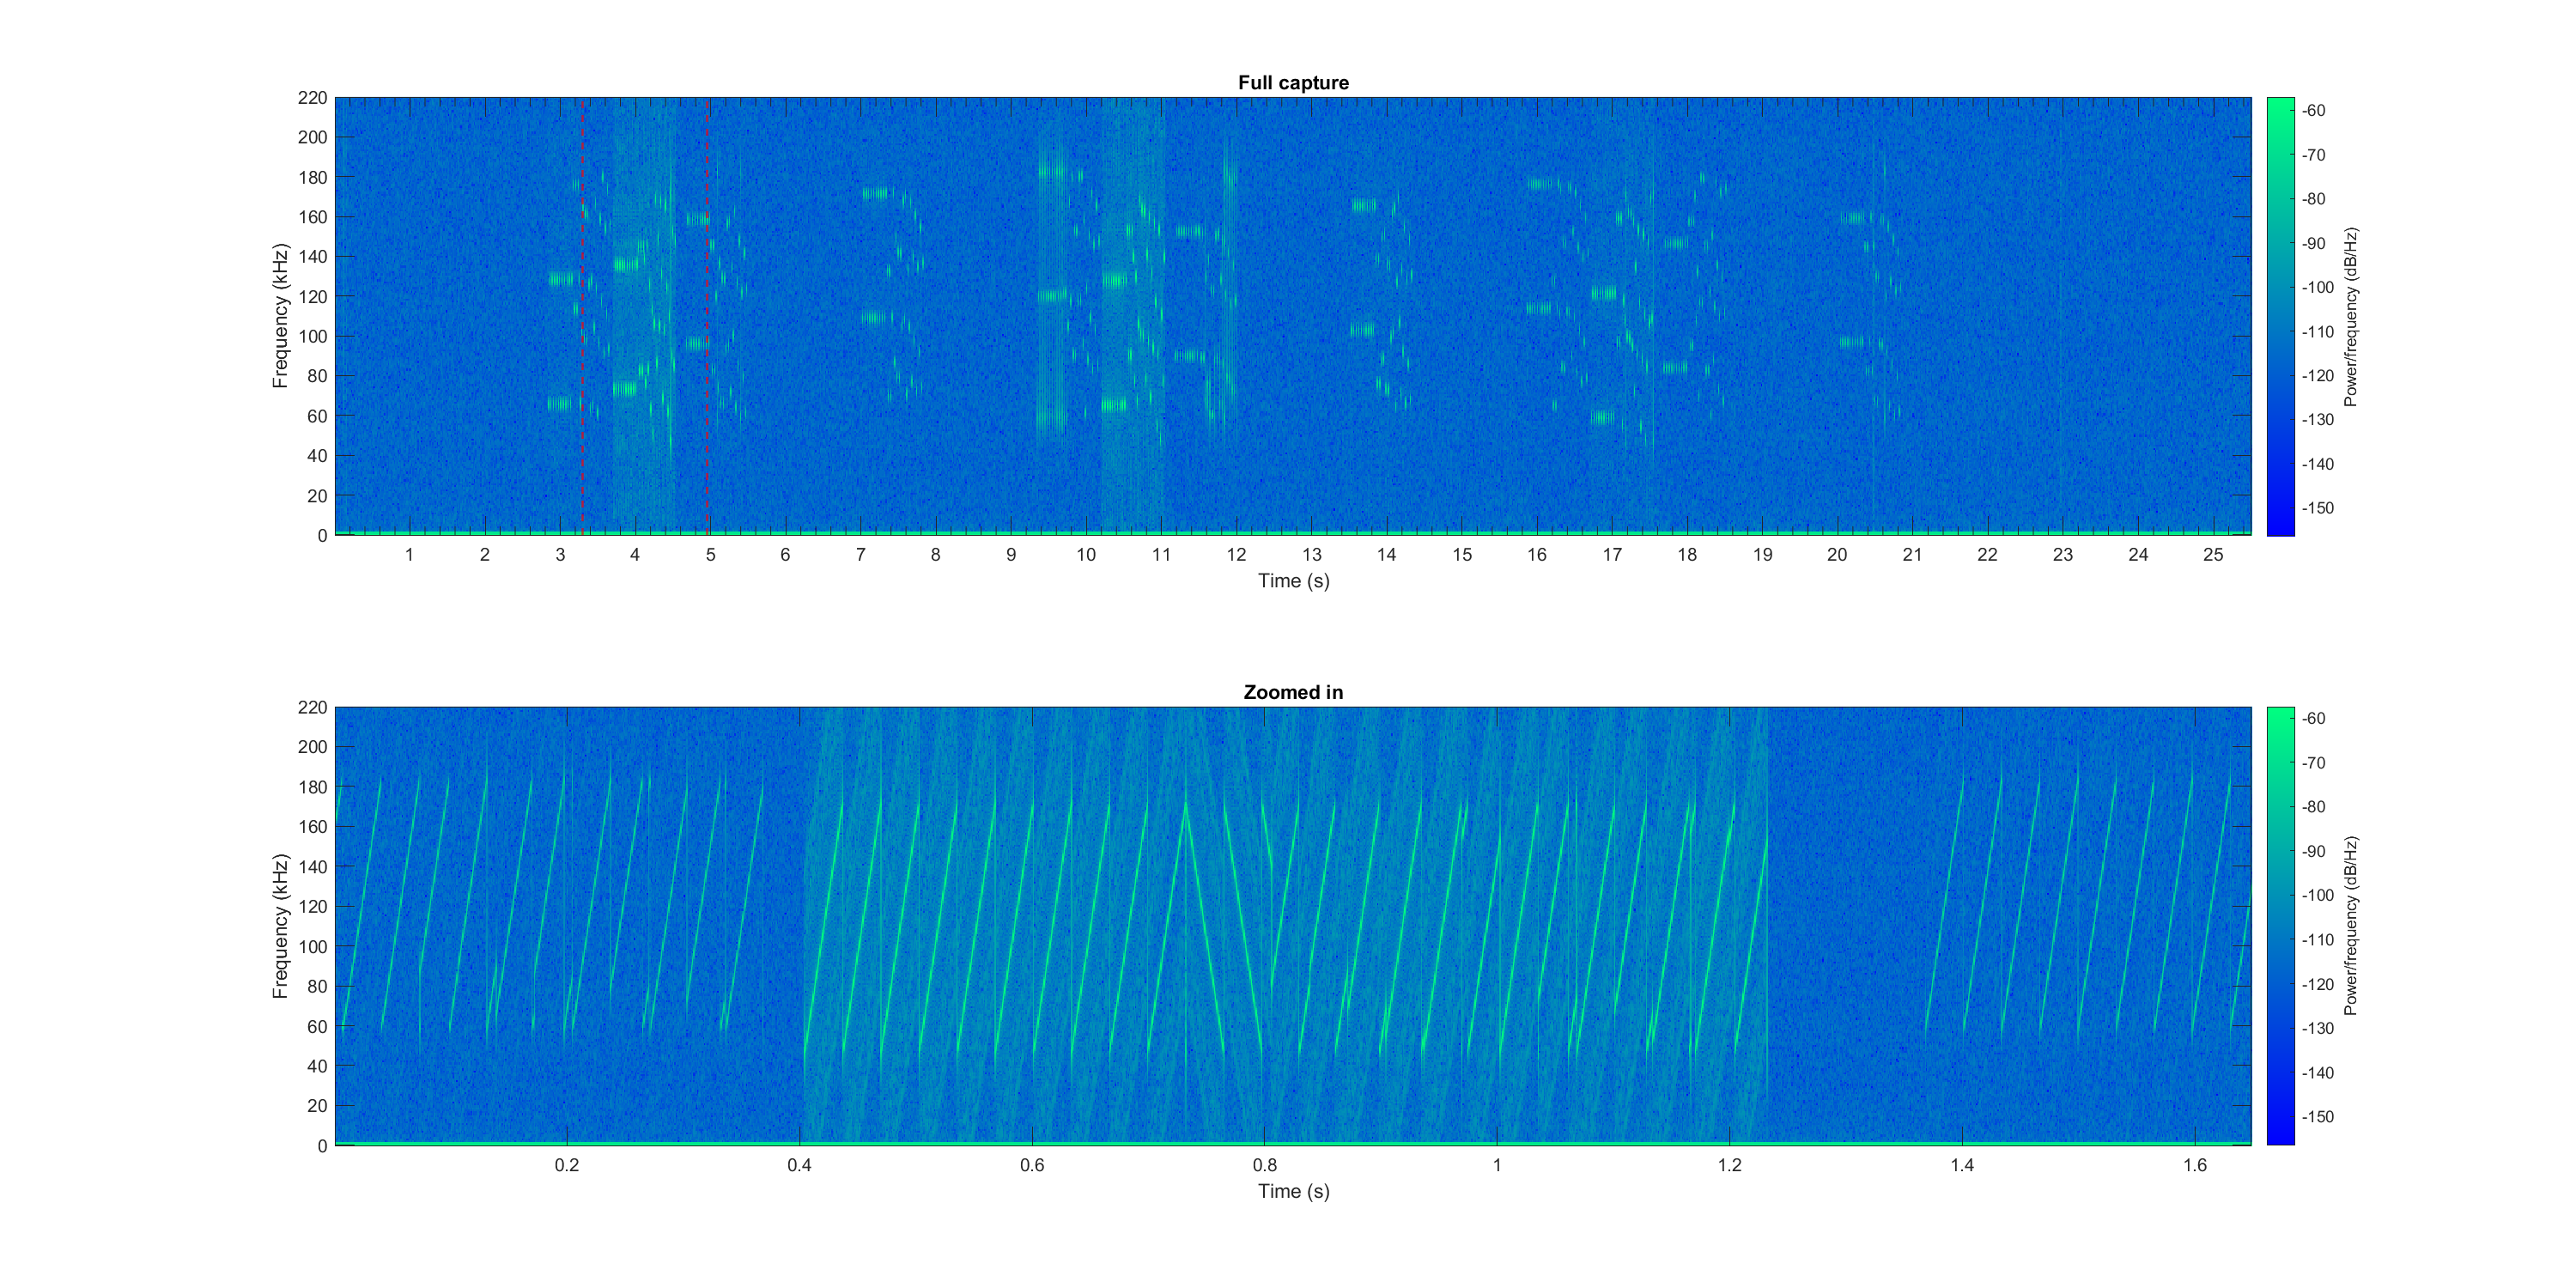
\includegraphics[width=\textwidth]{research/gqrx/zoom-win1024-sig1-lvl3}
    \caption{\label{img:signal1-level3}Spektrogram sygnałów z~pierwszej próbki wraz ze zbliżeniem między 3.4s a 5s}
\end{figure}

\begin{figure}[!htbp]
    \centering
    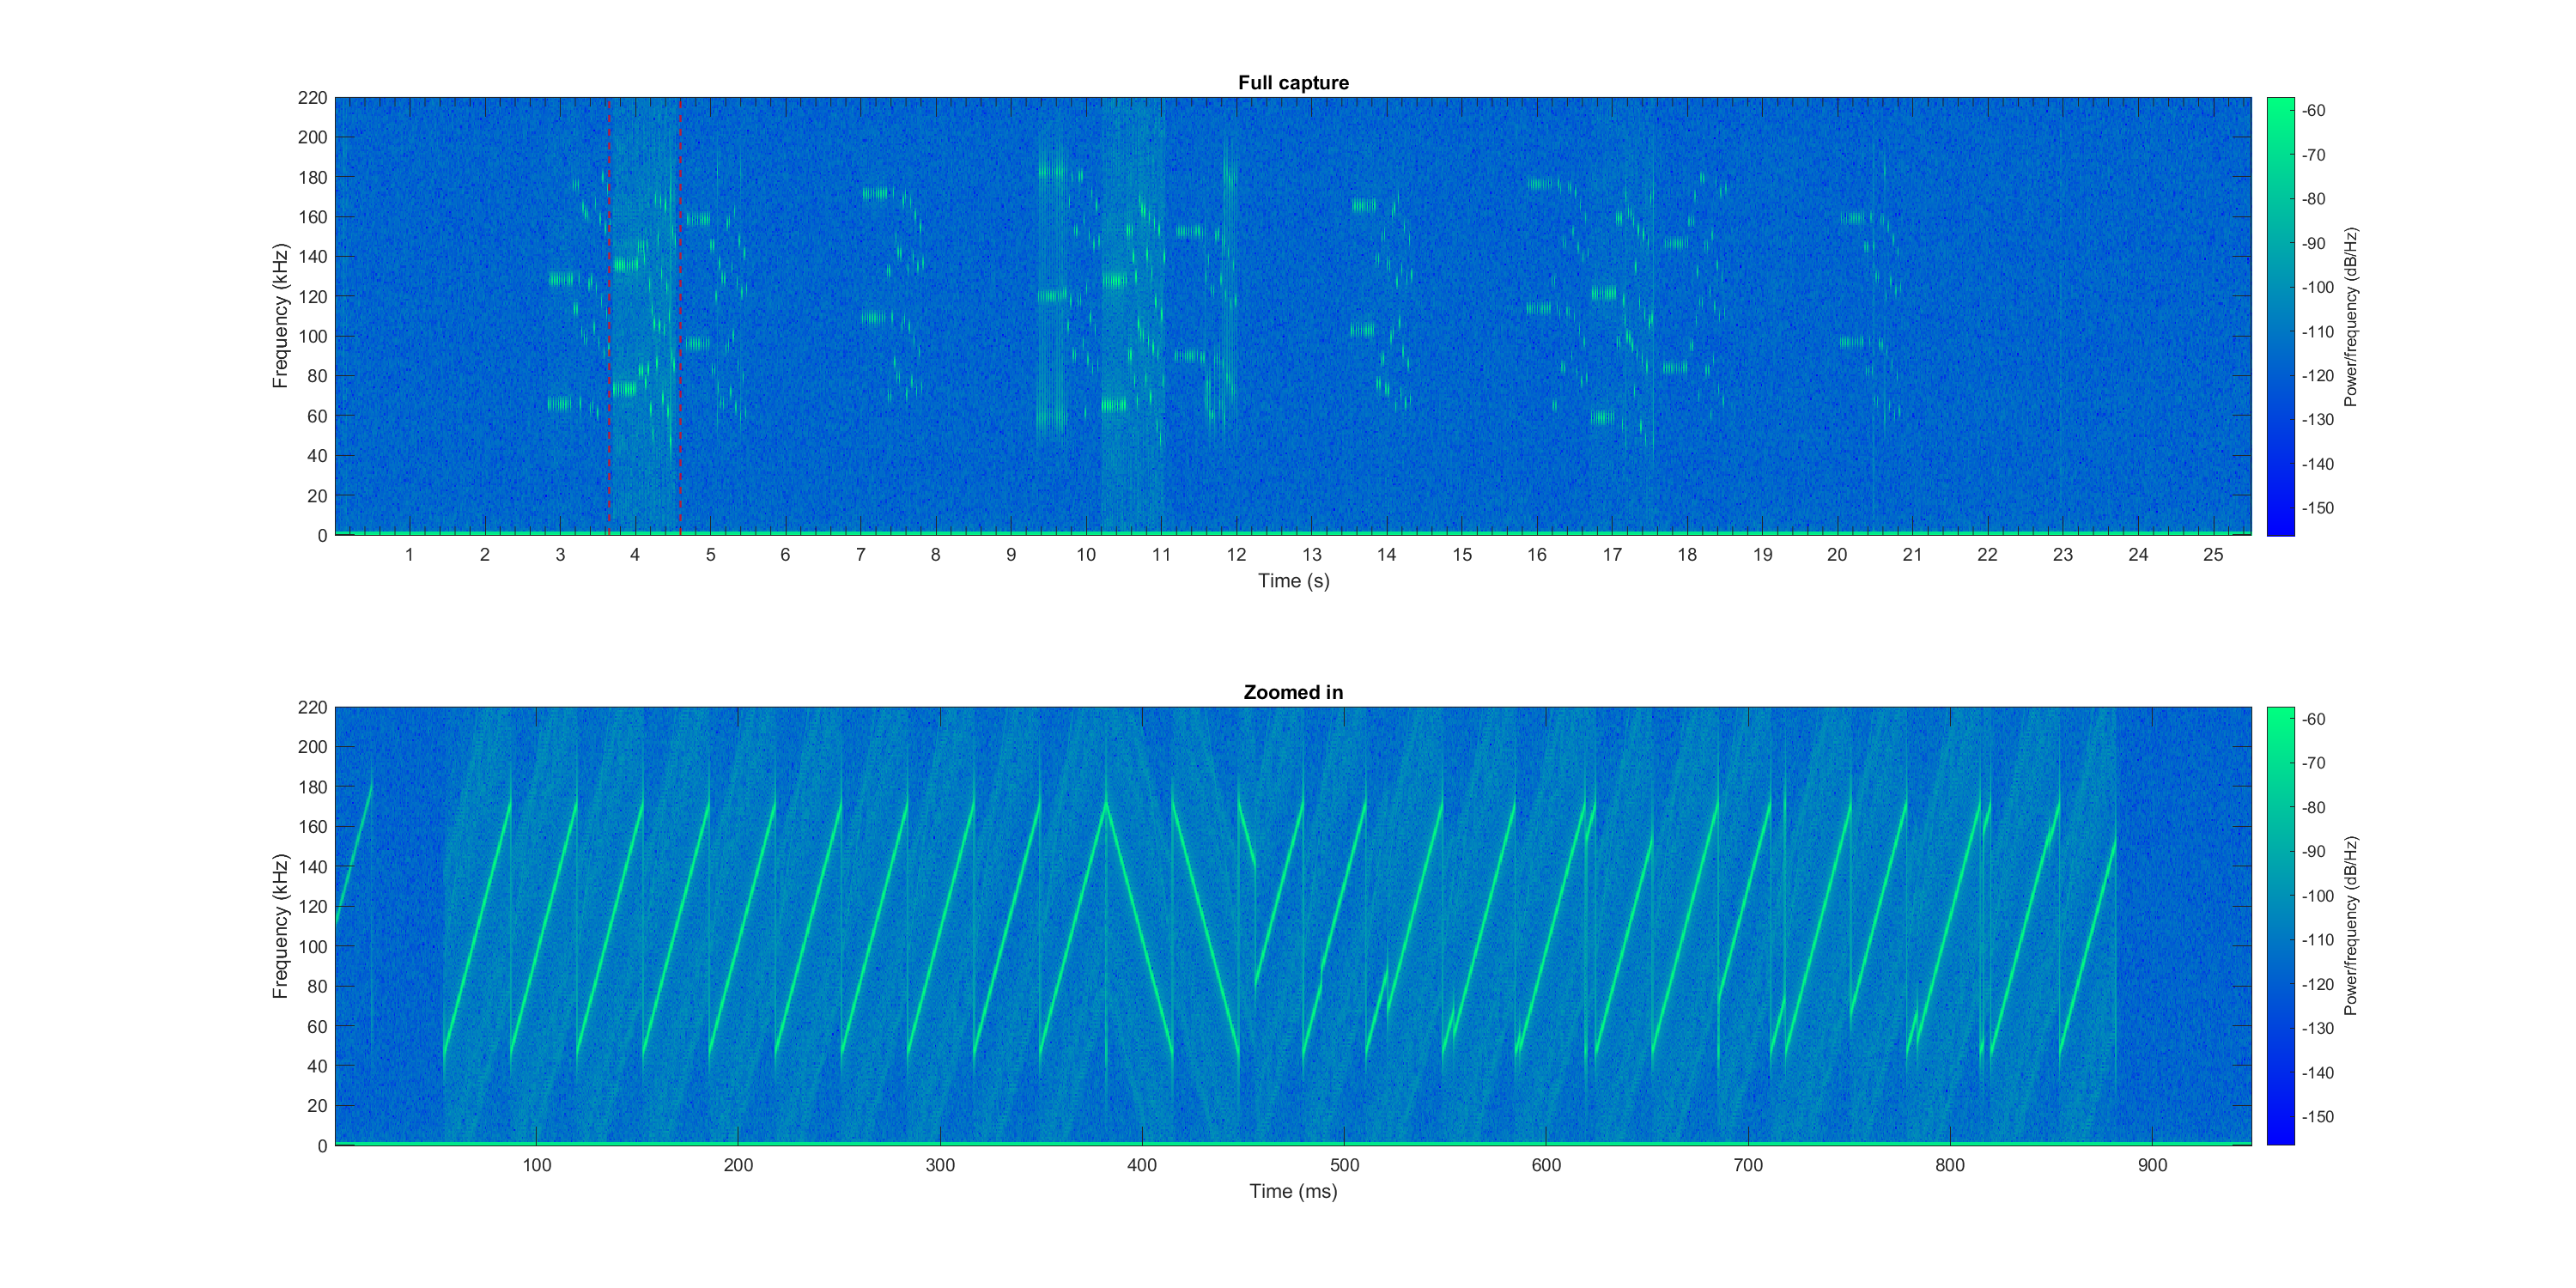
\includegraphics[width=\textwidth]{research/gqrx/zoom-win1024-sig1-lvl4}
    \caption{\label{img:signal1-level4}Spektrogram sygnałów z~pierwszej próbki wraz ze zbliżeniem między 3.6s a 4.6s,
        widoczna jedna transmisja}
\end{figure}

Na podstawie wygenerowanych spektrogramów możliwe było przeanalizowanie jednej pełnej ramki transmisji danych. Dzięki
uzyskanemu dużemu przybliżeniu na analizowany sygnał możliwe było wyznaczenie granic poszczególnych elementów ramki
LoRa. Przedstawione zostało to na rys. \ref{img:signal2-zoomed-analysis} oraz \ref{img:signal3-zoomed-analysis}
(odpowiednio dla fragmentu z~zarejestrowanych próbek drugiej oraz trzeciej).

\begin{figure}[!htbp]
    \centering
    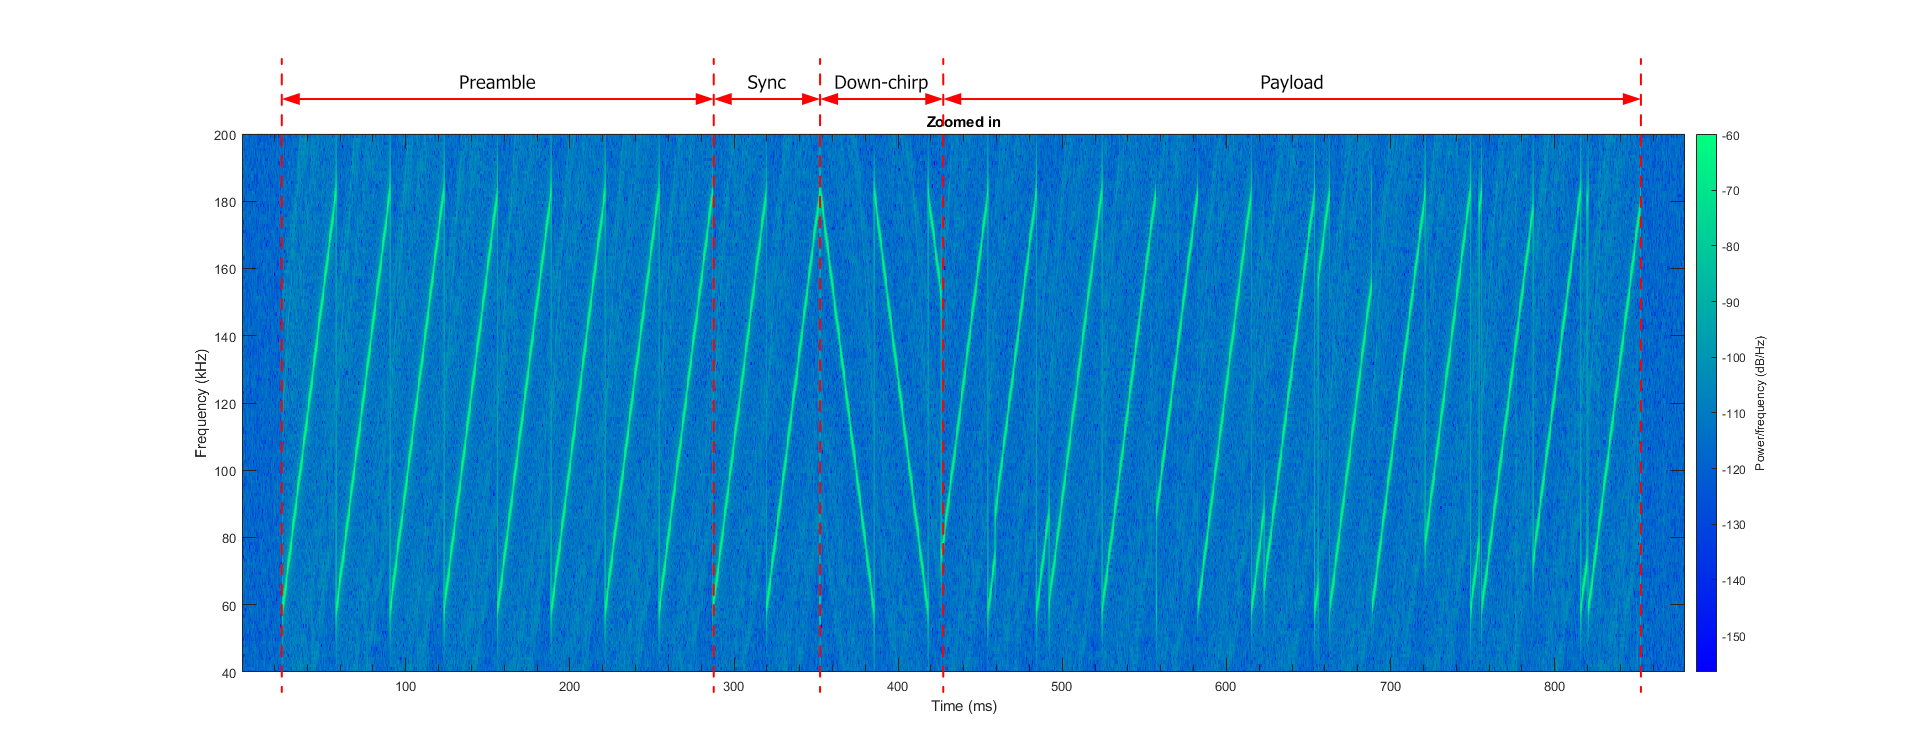
\includegraphics[width=\textwidth]{research/signal2-zoomed-analysis}
    \caption{\label{img:signal2-zoomed-analysis}Fragment drugiej próbki sygnału z~oznaczonymi poszczególnymi elementami
        ramki LoRa}
\end{figure}

\begin{figure}[!htbp]
    \centering
    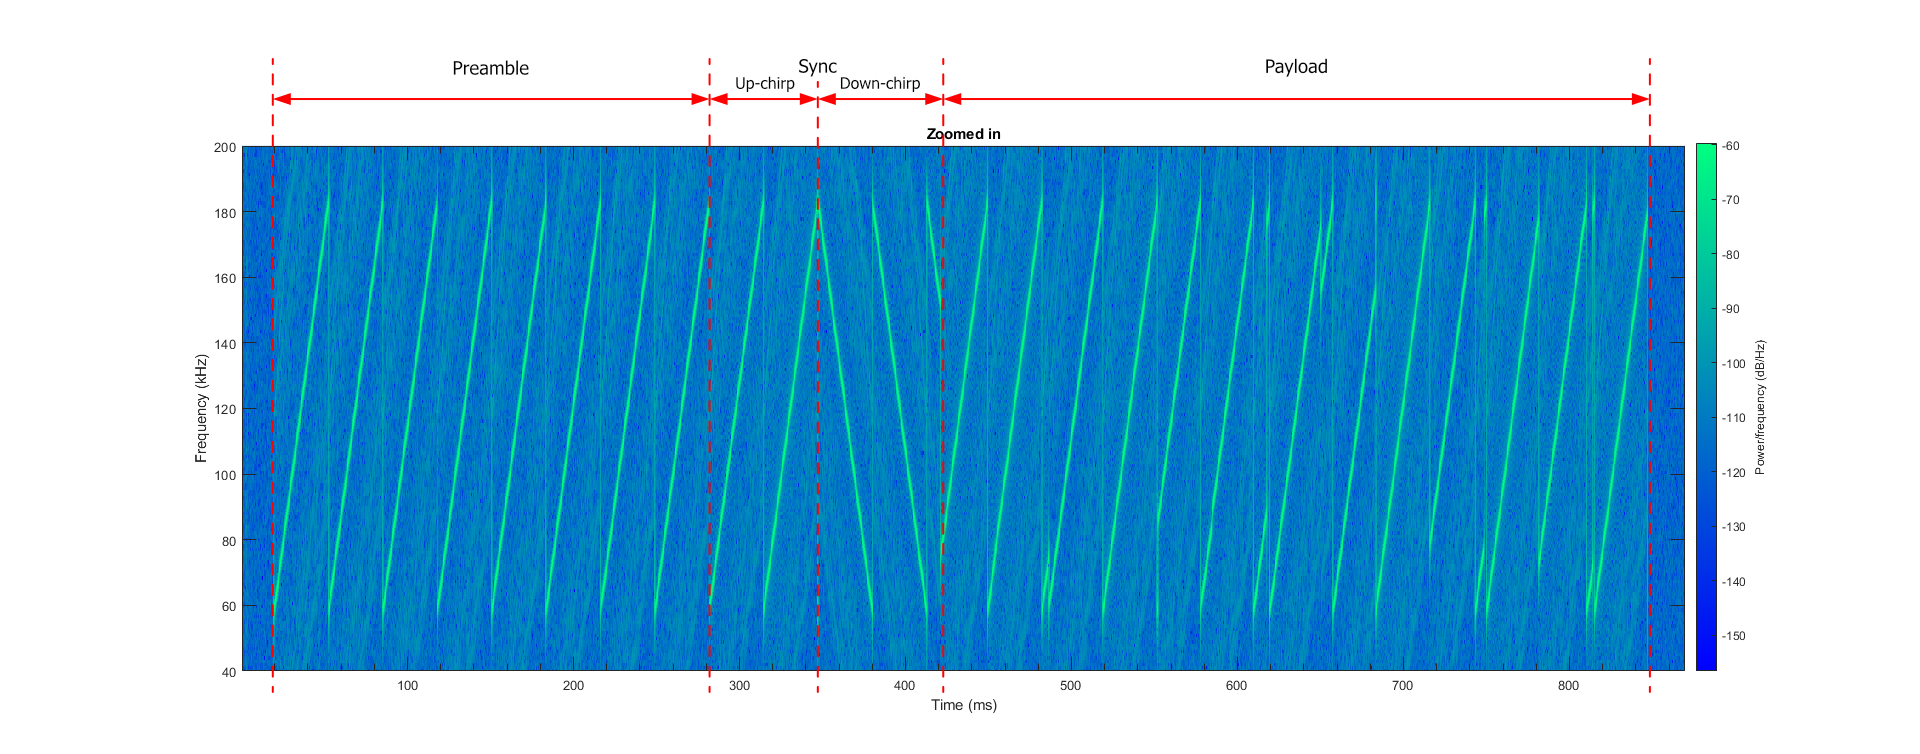
\includegraphics[width=\textwidth]{research/signal3-zoomed-analysis}
    \caption{\label{img:signal3-zoomed-analysis}Fragment trzeciej próbki sygnału z~oznaczonymi poszczególnymi elementami
        ramki LoRa}
\end{figure}

\FloatBarrier
Na przedstawionych fragmentach spektrogramów widoczne są różnice, pokazujące, że możliwe jest w~pewnym stopniu
rozróżnienie elementów transmisji. Są one widoczne tylko w~częściach oznaczonych jako "Payload" na wygenerowanych
wykresach, ponieważ tylko te elementy są zmienne w~każdej transmisji -- zawierają nagłówek, właściwe przesyłane dane
oraz kod CRC (ang. \textsl{Cyclic Redundancy Check}, służący wykrywaniu potencjalnych błędów w~transmisji). Pozostałe
elementy są elementami stałymi dla każdej ramki: preambuła (której długość ustawiona została na 8~symboli) -- pozwala
innym elementom sieci na wykrycie początku transmisji ramki, a~także dodatkowe symbole up-chirp oraz down-chirp --
w~sumie 4.25 symbolu, służące synchronizacji, aby mieć jak największą pewność, że dane, które mają zostać przesłane, nie
zostaną w~żaden sposób zniekształcone przez ew. przesunięcia w~czasie.

Ponieważ każda ramka LoRa zawiera kodowanie, możliwe jest jedynie rozróżnienia pojedynczych ramek między sobą, jednakże
nie jest już możliwe, korzystając wyłącznie ze spektrogramów, rozpoznanie co w~danym momencie jest przesyłane.
W~zaprezentowanych ramkach z~dwóch różnych próbek widać pewne różnice w~przesyłanych symbolach, jednakże tylko na
podstawie tego nie jest możliwe pokazanie, które symbole przedstawiają konkretne bity przesyłanych wiadomości.
